%\documentclass[10pt,reqno]{amsart}
\documentclass[sn-mathphys-num]{sn-jnl}

%\setlength{\topmargin}{0cm}
%\setlength{\textheight}{21cm}
%\setlength{\oddsidemargin}{0in}
%\setlength{\evensidemargin}{0in}
%\setlength{\textwidth}{6.5in}
%\setlength{\parindent}{.25in}

%\pagestyle{plain}
\usepackage{stmaryrd}
\usepackage{amssymb, amsmath, amsthm}
\usepackage{mathtools}
\usepackage{xcolor}
\usepackage{hyperref}
%\usepackage{showkeys}
\usepackage{enumerate}
\usepackage{subfig}
\usepackage{enumitem} 
\usepackage{todonotes}
\usepackage{booktabs}
\usepackage[]{algorithm2e}
\usepackage[capitalize]{cleveref}
\usepackage{placeins}
\crefname{equation}{}{}
\usepackage{verbatim}
\usepackage{bbm}

%\usepackage{graphicx}
%% expansion of width
%\textwidth=15.7cm
%\textheight=22.5cm
%\parskip=3pt
%\parindent=8mm
%\oddsidemargin=2mm
%\evensidemargin=0mm
%\topmargin=-0.5cm
%\marginparwidth=1cm


%% definition of theorem-type environments
\newtheorem{thm}{Theorem}[section]
\newtheorem{lem}[thm]{Lemma}
\newtheorem{cor}[thm]{Corollary}
\newtheorem{prop}[thm]{Proposition}
\newtheorem{defn}[thm]{Definition}
\newtheorem{rmk}{Remark}
\newtheorem{exa}{Example}
\newtheorem{assum}{Assumption}
\numberwithin{equation}{section}
\newcommand{\bel}{\begin{equation} \label}
\newcommand{\ee}{\end{equation}}
\def\beq{\begin{equation}}
\def\eeq{\end{equation}}
\newcommand{\jump}[1]{\llbracket#1\rrbracket}
\newcommand{\bea}{\begin{eqnarray}}
\newcommand{\eea}{\end{eqnarray}}
\newcommand{\beas}{\begin{eqnarray*}}
\newcommand{\eeas}{\end{eqnarray*}}
\newcommand{\pd}{\partial}
\newcommand{\mdiv}[1]{\ensuremath{\mathrm{div} \left( #1 \right)}}
\newcommand{\dd}{\mbox{d}}

\newcommand{\ep}{\varepsilon}
\newcommand{\la}{\lambda}
\newcommand{\va}{\varphi}
\newcommand{\ppp}{\partial}
\newcommand{\chch}{\chi_{\eta}}
\newcommand{\walpha}{\widetilde{\alpha}}
\newcommand{\wbeta}{\widetilde{\beta}}

\newcommand{\re}{\mathfrak R}

\newcommand{\im}{\mathfrak I}
\newcommand{\pdif}[2]{\frac{\partial #1}{\partial #2}}
\newcommand{\ppdif}[2]{\frac{\partial^2 #1}{{\partial #2}^2}}
\newcommand{\R}{\mathbb{R}}
\newcommand{\C}{\mathbb{C}} 
\newcommand{\N}{\mathbb{N}} 
\newcommand{\ooo}{\overline}
\newcommand{\uu}{\mathbf{u}}
\renewcommand{\v}{\mathbf{v}}
\newcommand{\y}{\mathbf{y}}
\newcommand{\RR}{\mathbf{R}}
\newcommand{\Y}{\mathbf{Y}}
\newcommand{\w}{\mathbf{w}}
\newcommand{\z}{\mathbf{z}}
\newcommand{\G}{\mathbf{G}}
\newcommand{\cB}{\mathcal{B}}
\newcommand{\cD}{\mathcal{D}}
\newcommand{\cL}{\mathcal{L}}
\newcommand{\cO}{\mathcal{O}}
\newcommand{\Hin}{\mathcal{H}_{\mathrm{in},T_0}}
\newcommand{\Gi}{S_{\mathrm{in}}}
\newcommand{\Go}{S_{\mathrm{out}}}
\newcommand{\dom}{\mathrm{Dom}}

\newcommand{\sdd}{\mathcal{E}}


\renewcommand{\baselinestretch}{1.5}
%
\renewcommand{\div}{\mathrm{div}\,}  %div
\newcommand{\grad}{\mathrm{grad}\,}  %grad
\newcommand{\rot}{\mathrm{rot}\,}  %rot

\newcommand{\supp}{\mathrm{supp}\,}  %supp
%\newcommand{\span}{\mathrm{span}\,} %span

\allowdisplaybreaks
%%  item
\renewcommand{\theenumi}{\arabic{enumi}}
\renewcommand{\labelenumi}{(\theenumi)}
\renewcommand{\theenumii}{\alph{enumii}}
\renewcommand{\labelenumii}{(\theenumii)}
\def\epsilon{\varepsilon}
%\def\phi {\varphi}
\def \la {{\lambda}}
\def \a {{\alpha}}
\def\t{\theta}
\def\fh{\frac{1}{h}}


\DeclareMathOperator{\dis}{dist}


\newcommand{\wop}{\square_c}

\newcommand{\tnorm}[1]{\vert\hspace{-0.3mm}\Vert#1\Vert\hspace{-0.3mm}\vert}

\providecommand{\abs}[1]{\left\lvert#1\right\rvert}
% pour les normes
\providecommand{\norm}[1]{\left\lVert#1\right\rVert}

\renewcommand{\leq}{\leqslant}
\renewcommand{\geq}{\geqslant}
\providecommand{\abs}[1]{\left\lvert#1\right\rvert}
% pour les normes
\providecommand{\norm}[1]{\left\lVert#1\right\rVert}
\def\thefootnote{{}}



\newcommand{\HOX}[1]{\marginpar{\footnotesize #1}}

\newcommand{\gammaGLS}{\gamma_{\text{GLS}}}
\newcommand{\gammaCIP}{\gamma}

\newcommand{\dT}{\mathrm{d}t}
\newcommand{\dX}{\mathrm{d}x}
\newcommand{\dS}{\mathrm{d}S}

\newcommand{\STdom}{Q}

\newcommand{\STdata}{\omega_T}
\newcommand{\STdataDisc}{\underline{\omega}_T}
\newcommand{\SemiDiscSpace}{\mathcal{W}_h}
\newcommand{\FullyDiscSpace}{W}

%\newcommand{\FullyDiscrSpaceDisc}[2]{ W_{ {#1},{#2}}^{ \text{dc} } }
%\newcommand{\FullyDiscrSpaceCont}[2]{ W_{ {#1},{#2}}^{ \text{c}  } }
%\newcommand{\ProdFullyDiscrSpaceDisc}[2]{  \mathcal{W}_{ {#1},{#2} }^{ \text{dc} } }
%\newcommand{\ProdFullyDiscrSpaceCont}[1]{  \mathcal{W}_{ {#1} }^{ \text{c} } }

\newcommand{\SemiDiscrSpace}[1]{ W^{ {#1}}_{h} }
\newcommand{\ProdSemiDiscrSpace}[1]{ \mathcal{W}^{ {#1} }_{h} }
\newcommand{\FullyDiscrSpace}[2]{ W^{ {#1},{#2}}_{h, \Delta t  } }
\newcommand{\FullyDiscrSpaceHat}[2]{ \hat{W}^{ {#1},{#2}}_{h, \Delta t  } }
\newcommand{\ProdFullyDiscrSpace}[2]{ \mathcal{W}^{ {#1},{#2}}_{h, \Delta t  } }

\DeclarePairedDelimiterX{\inp}[2]{(}{)}{#1, #2}
\newcommand{\tangular}[1]{ \llbracket\kern-0.5ex|#1|\kern-0.5ex\rrbracket} 
%\newcommand{\jump}[1]{\llbracket#1\rrbracket}
\newcommand{\avg}[1]{ \{\!\!\{#1\}\!\!\}}

\newboolean{includeextras}
\ifdefined\withextras
\setboolean{includeextras}{true}
\else
\setboolean{includeextras}{false}
\fi

\newcommand{\putextra}[1]{\ifthenelse{\boolean{includeextras}}{#1}{}}

\newcommand{\Uh}{\underline{\mathbf{U}}_h}
\newcommand{\Vh}{\underline{\mathbf{V}}_h}
\newcommand{\Yh}{\underline{\mathbf{Y}}_h}
\newcommand{\Zh}{\underline{\mathbf{Z}}_h}
\newcommand{\Wh}{\underline{\mathbf{W}}_h}

\newcommand{\ul}{\underline{u}}
\newcommand{\yl}{\underline{y}}
\newcommand{\zl}{\underline{z}}
\newcommand{\wl}{\underline{w}}

\newcommand{\Sud}{S^{\uparrow \downarrow}_{\Delta t}}


\newcommand{\dt}{\partial_t}
\newcommand{\dtt}{\partial_t^2}

%%% TvB: Added for plots, some might be redundant ##

%------------------------- Added for Plots ----
% Tikz package
\usepackage{tikz}
\usepackage{pgfplots,pgfplotstable}
\usepgfplotslibrary{colorbrewer,groupplots}
\usepackage{caption}
\pgfplotsset{compat=1.18}


%find colors at https://colorbrewer2.org/#type=qualitative&scheme=Set1&n=5
\pgfplotsset{
% initialize Set1-5:
cycle list/Set1-5,
% combine it with ’mark list*’:
cycle multiindex* list={
mark list*\nextlist
Set1-5\nextlist
},
}

\pgfplotsset{
    discard if not/.style 2 args={
        x filter/.append code={
            \edef\tempa{\thisrow{#1}}
            \edef\tempb{#2}
            \ifx\tempa\tempb
            \else
                \def\pgfmathresult{inf}
            \fi
        }
    }
}

%%%

\providecommand{\jp}[1]{\newline {\color{cyan} \hspace*{-0.5cm} $\rightsquigarrow$ \underline{\textbf{JP:}} \textit{#1} \newline}}

\date{\today}
\begin{document}

\title{A numerical study of variational data assimilation for the wave equation in heterogeneous media}

\author[1]{\fnm{Erik} \sur{Burman}}\email{e.burman@ucl.ac.uk}
\author[1]{\fnm{Janosch} \sur{Preuss}}\email{j.preuss@ucl.ac.uk}
\author[2]{\fnm{Tim} \sur{van Beeck}}\email{t.beeck@math.uni-goettingen.de}

\affil[1]{\orgdiv{Department of Mathematics}, \orgname{University College London}, \orgaddress{\street{Gower Street}, \city{London}, \postcode{WC1E 6BT}, \country{United Kingdom}}}

\affil[2]{\orgdiv{Institute for Numerical and Applied Mathematics}, \orgname{University of G\"{o}ttingen}, \orgaddress{\street{Lotzestr. 16-18}, \city{G\"{o}ttingen}, \postcode{37083}, \country{Germany}}}

\abstract{In recent years several numerical methods for solving the unique continuation problem for the wave equation in a homogeneous medium with given data on the lateral boundary of the space-time cylinder have been proposed. Under these conditions the problem enjoys Lipschitz stability which allows to devise optimally convergent numerical methods. In this article we investigate whether these results carry over to the case in which the medium exhibits a jump discontinuity. Our numerical experiments suggest a positive answer provided that the geometric control condition is satisfied. However, we also observe that the presence of discontinuities in the medium renders the computations far more demanding than in the homogeneous case.
}

\keywords{Unique continuation, data assimilation, wave equation, discontinuous coefficients, geometric control condition}

\maketitle

\section{Introduction}
\noindent In this article, we consider the discretization of a data assimilation problem for the wave equation in heterogeneous media. In the following, let $\Omega \subset \mathbb{R}^d$ be a bounded domain with smooth boundary $\partial \Omega$. We assume that $\Omega$ is split by a smooth $(d-1)$-dimensional 
interface $\Gamma$ into two disjoint components, i.e.\ $\Omega \setminus \Gamma = \Omega_1 \cup 
\Omega_2$ and $\Omega_1 \cap \Omega_2 = \emptyset$.
 We consider a scalar wave speed
\[
 c(x) := \begin{cases}
       c_1(x),  & x \in \Omega_1, \\
        c_2(x), & x \in \Omega_2,
    \end{cases}
    \quad 
    \text{ with } c_i \in C^\infty(\Omega_i), \; i = 1,2,
\]
 %$c(x) = \mathbbm{1}_{\Omega_1} c_1(x) + \mathbbm{1}_{\Omega_2} c_2(x)$, $c_i \in C^\infty(\Omega_i)$, $i = 1,2$,
which may be discontinuous across the interface $\Gamma$, but constant in time. For a final time $T > 0$, we consider the space-time domain $Q = (0,T) \times \Omega$ with lateral boundary $\Sigma \coloneqq (0,T) \times \partial \Omega$. For any nonempty subset $\omega \subset \Omega$, we set $\omega_T \coloneqq (0,T) \times \omega$. In the following, let $\wop$ be the wave operator with discontinuous wave-speed defined as 
\begin{equation*}
    \wop u := \partial_t^2 - \div(c^2 \nabla u).
\end{equation*}
In particular, we write $\square_1$ if $c_i = 1$, $i = 1,2$, i.e. if we are considering the case of homogeneous media. 
Then, we consider the problem: find $u : Q \rightarrow \mathbb{R}$ such that 
\begin{equation}\label{eq:waveEquation}
        (\wop u, u) = (0,0) \quad \text{ in } Q \times \Sigma,
\end{equation}
along with the natural interface conditions 
\begin{equation}\label{eq:IF-conditions}
	\jump{u}_{\Gamma} = 0 \text{ on } \Sigma, \qquad 
	\quad \jump{c^2 \nabla u}_{\Gamma} \cdot \mathbf{n}_{\Gamma} = 0 \text{ on } \Sigma, 
\end{equation}
where $\mathbf{n}_{\Gamma}$ is the normal vector on $\Gamma$ pointing into $\Omega_+$ 
and the jump across $\Gamma$ is defined\textsuperscript{1}\footnotemark \footnotetext{\textsuperscript{1}And anologously for vector-valued functions.} as $\jump{u}_{\Gamma} = u_{+}-u_{-}$ with $u_{\pm}$ being the traces 
of $u|_{\Omega_{\pm}}$ on $\Gamma$. \par 
\noindent To ensure that the problem is well posed, one usually prescribes initial data
\begin{equation}\label{eq:initialData}
    (u,\dt u) \vert_{t = 0} = (u_0,u_1) \text{ in } \Omega, \tag{IVP} 
\end{equation}
where $u_0 \in H^1(Q)$ and $u_1 \in L^2(Q)$ are given. For a detailed analysis of the well-posedness of the problem \eqref{eq:waveEquation}-\eqref{eq:IF-conditions}+\eqref{eq:initialData} in heterogeneous media we refer to \cite{StolkPhD}. 
Here we consider a data assimilation problem instead, i.e. we assume that the initial data is unknown and that there are given measurements $u_{\omega} \in L^2(\omega_T)$ which are prescribed in a data domain $\omega_T$, $\omega \subset \Omega$, $\omega \not = \emptyset$:
\begin{equation}\label{eq:dataMatch}
    u = u_{\omega} \text{ in } \omega_T. \tag{DA}
\end{equation}


%\noindent In a homogeneous medium, where $c_i = 1$, $i = 1,2$,
\noindent In a medium without an interface the problem \eqref{eq:waveEquation}+\eqref{eq:dataMatch} is well-studied, see e.g.~References \cite{CM15,BFO20,BFMO21,MM21,DMS23,BDE24}. In particular, it is known that if $c_i = 1$, $i = 1,2$, the boundary $\partial \Omega$ is strictly convex and the set $\omega_T \subset Q$ fulfills the geometric control condition (GCC) \cite{BLR92}, then the problem is Lipschitz stable. Roughly speaking, a set $\omega \subset \Omega$ and a final time $T$ fulfill the GCC if all geometric optic rays traveling with unit speed\textsuperscript{2}\footnotemark \footnotetext{\textsuperscript{2}with adapting the metric to the wave speed $c$.} in $\Omega$, taking into account possible reflections on the boundary $\partial \Omega$, intersect the set $(0,T) \times \omega$. For a precise definition, we refer to \cite{BLR92}. Assuming that the GCC is satisfied, we have the following result.

\begin{thm}\label{thm:Lipschitz}
    Assume that $c_i = 1$, $i = 1,2$, and that $\partial \Omega$ is stricly convex. If $\omega_T \subset Q$ fulfills the GCC, then there exists a constant $C > 0$ such that for any $\phi \in H^1(Q)$ we have the following estimates
    \begin{align*}
        \Vert \phi \Vert_{L^\infty(0,T;L^2(\Omega))} + \Vert \dt \phi \Vert_{L^2(0,T;H^{-1}(\Omega))} &\le C \left(  \Vert \phi \Vert_{L^2(\omega_T)} + \Vert \phi \Vert_{L^2(\Sigma)} + \Vert \square_1 \phi \Vert_{H^{-1}(Q)} \right), \\
        \Vert \phi \vert_{t = 0} \Vert_{L^2(\Omega)} + \Vert \dt \phi \vert_{t = 0} \Vert_{H^{-1}(\Omega)} &\le C \left(\Vert \phi \Vert_{L^2(\omega_T)} + \Vert \phi \Vert_{L^2(\Sigma)} + \Vert \square_1 \phi \Vert_{H^{-1}(Q)} \right). 
    \end{align*}
\end{thm}

\begin{proof}
    See \cite[Thm. A.4]{BFMO21control} and \cite[Rem. A.5]{BFMO21control}.
\end{proof}

\noindent For the heterogeneous case where $c_1 \not =  c_2$, the problem is less studied. In the absence of the GCC, we have to assume that the final time $T$ is large enough to ensure that problem \eqref{eq:waveEquation}-\eqref{eq:IF-conditions}+\eqref{eq:dataMatch} is well-posed. To be precise, Holmgren's unique continuation theorem guarantees that \eqref{eq:waveEquation}-\eqref{eq:IF-conditions}+\eqref{eq:dataMatch} is uniquely solvable if
\begin{equation}\label{eq:Tcondition}
    T > 2 \sup_{x \in \Omega} \operatorname{dist}_{c}(x,\omega_T),
\end{equation}
where $\operatorname{dist}_c(x,\omega_T) := \inf_{y \in \omega_T} d_c(x,y)$ with $d_c$ being the distance function defined as the length of the shortest continuous path in $\Omega$ connecting $x$ and $y$ with respect to the metric adapted to the discontinuous wave speed $c$. While the condition \eqref{eq:Tcondition} guarantees unique solvability, the stability of problem \eqref{eq:waveEquation}-\eqref{eq:IF-conditions}+\eqref{eq:dataMatch} can be poor. It has been shown in \cite[Thm. 5.19]{Filippas22} that under the assumption \eqref{eq:Tcondition} the following stability result holds:  
\begin{thm}[Thm. 5.19 of \cite{Filippas22}]\label{thm:filippas}
    Let $\omega_T \subset \Omega$ be nonempty and let $T$ be s.t. \eqref{eq:Tcondition} holds. Then, there exists $C,\kappa$ such that for any initial data $(u_0,u_1) \in H^1_0(\Omega) \times L^2(\Omega)$ and $u$ solving \eqref{eq:IF-conditions}+\eqref{eq:initialData} and  
\[
\wop u \in L^2(Q), \quad u = 0 \text{ on } \Sigma,
\]
one has for any $\mu > 0$ that 
    \begin{equation}\label{eq:FilippasEstimate}
        \Vert (u_0,u_1) \Vert_{L^2 \times H^{-1}} \le C e^{\kappa \mu} \left( \Vert u \Vert_{L^2(\omega_T)} + \Vert \wop u \Vert_{L^2(Q)} \right) + \frac{C}{\mu} \Vert (u_0,u_1) \Vert_{H^1 \times L^2}. 
    \end{equation}
    In particular, if $(u_0,u_1) \not = (0,0)$ we have that 
    \begin{equation}\label{eq:FilippasEstimateLog}
        \Vert (u_0,u_1) \Vert_{L^2 \times H^{-1}} \le C \frac{\Vert (u_0,u_1) \Vert_{H^1 \times L^2}}{\log \left( 1 + \frac{\Vert (u_0,u_1) \Vert_{H^1 \times L^2}}{ \Vert u \Vert_{L^2(\omega_T)} + \Vert \wop u \Vert_{L^2(Q)}} \right)}. 
    \end{equation} 
\end{thm} 

\noindent In this article, we introduce a discontinuous in time finite element method to solve the data assimilation problem \eqref{eq:waveEquation}-\eqref{eq:IF-conditions}+\eqref{eq:dataMatch} in the heterogeneous case. In particular, we want to investigate numerically if the following assumption, motivated by Thm. \ref{thm:Lipschitz} for the homogeneous case, is justified. 

\begin{assum}\label{assum:LipschitzStability}
    If $\omega_T \subset Q$ fulfills the GCC, then there exists a constant $C > 0$ such that for any $\phi \in H^1(Q)$ we have the following estimates
    \begin{align*}
        \Vert \phi \Vert_{L^\infty(0,T;L^2(\Omega))} + \Vert \dt \phi \Vert_{L^2(0,T;H^{-1}(\Omega))} &\le C \left(  \Vert \phi \Vert_{L^2(\omega_T)} + \Vert \phi \Vert_{L^2(\Sigma)} + \Vert \square_c \phi \Vert_{H^{-1}(Q)} \right), \\
        \Vert \phi \vert_{t = 0} \Vert_{L^2(\Omega)} + \Vert \dt \phi \vert_{t = 0} \Vert_{H^{-1}(\Omega)} &\le C \left(\Vert \phi \Vert_{L^2(\omega_T)} + \Vert \phi \Vert_{L^2(\Sigma)} + \Vert \square_c \phi \Vert_{H^{-1}(Q)} \right). 
    \end{align*}
\end{assum}

That is, we would like to understand whether the Lipschitz stability property is preserved in presence of strong heterogeneity in the medium provided that the GCC holds. This question is of high practical importance since discontinuous media appear in many applications, e.g.\ in seismology. If the corresponding data assimilation problems were indeed subject to the poor logarithmic stability property ensured by \eqref{eq:FilippasEstimateLog}, this would pose an enormous challenge for the design of accurate and realiable numerical methods for their resolution.

\section{Discretization (fully discrete \& dG in time)} 
\noindent In this section, we introduce a fully discrete discontinuous in time finite element method to discretize the data assimilation problem \eqref{eq:waveEquation}-\eqref{eq:IF-conditions}+\eqref{eq:dataMatch} for the wave equation in heterogeneous media. The discretization is based on the scheme introduced in \cite{BP24} for the homogeneous case. Before introducing the method in Section \ref{sec:method}, we describe the geometric partition of the space-time domain $Q$ into time slabs in Section \ref{sec:spaceTimeDiscretization}. 

\subsection{Discretization of the space-time domain}\label{sec:spaceTimeDiscretization}
Let $\hat{\mathcal{T}}_h$ be a quasi-uniform triangulation with mesh size $h$ such that $\hat{\Omega}:= \cup_{K \in \hat{\mathcal{T}}_h} K $ contains $\Omega$, i.e.\ $\Omega \subset \hat{\Omega}$. Setting $\mathcal{T}_h := \{ K \cap \Omega \mid K \in  \hat{\mathcal{T}}_h \}$ then ensures that $\Omega = \cup_{K \in \mathcal{T}_h} K$ holds true.  
We recall from  \cite[Sec. 4.2]{BFMO21control} that the triangulation $\{ \hat{\mathcal{T}}_h \mid h > 0 \}$ can be constructed such that for $h$ small enough the following continuous trace inequality holds:  For all $v \in [H^1(K)]^d$ and $K \in \mathcal{T}_h$, we have
\begin{equation}\label{eq:traceInequality}
    \Vert v \Vert_{[L^2(\partial K)]^d} \le C \left(h^{-1/2} \Vert v \Vert_{[L^2(K)]^d} + h^{1/2} \Vert \nabla v \Vert_{[L^2(K)]^d} \right).  
\end{equation}
We assume in what follows additionally that the triangulation $\mathcal{T}_h$ fits the interface $\Gamma$ and the data domain $\omega$. An extension to allow for unfitted interfaces could be possible utilizing techniques we introduced for a stationary problem in \cite{BP23arxiv}, but is certainly beyond the scope of this article. 

\noindent For $k \ge 1$, we define the $H^1$-conforming finite element space 
\begin{equation}
    V_h^k := \{ v \in H^1(\Omega) : v \vert_{K} \in \mathcal{P}^k(K) \ \forall K \in \mathcal{T}_h \},
\end{equation}
where $\mathcal{P}^k(K)$ denotes the space of polynomials of degree at most $k \in \mathbb{N}$ on $K \in \mathcal{T}_h$. Furthermore, we partition the time axis into $N$ subinterals $I_n = (t_n,t_{n+1})$, $n = 0, \dots, N-1$, where $0 = t_0 \le t_1 \le \dots \le t_N = T$. We assume that the intervals are of equal length and denote $\Delta t = \vert t_{n+1} -t_n \vert$. Then, we partition of $Q$ and $\Sigma$ into time-slabs 
\begin{equation}
    \begin{aligned}
        Q^n := &I_n \times \Omega, \quad \Sigma^n := I_n \times \Sigma, \quad n = 0, \dots, N-1, \\
        Q = &\bigcup_{n = 0}^{N-1} Q^n, \quad \phantom{:} \Sigma = \bigcup_{n = 0}^{N-1} \Sigma^n.
    \end{aligned}
\end{equation}
In the following, we denote the space-time integrals on the time slabs as 
\begin{equation*}
    (u,v)_{Q^n} := \int_{I_n} \int_{\Omega} uv \ \dX \dT, \quad (u,v)_{\Sigma^n} := \int_{I_n} \int_{\Sigma} uv \ \dS \dT,
\end{equation*}
and define $\Vert v \Vert^2_{Q^n} := (v,v)_{Q^n}$ and $\Vert v \Vert^2_{\Sigma^n} := (v,v)_{\Sigma^n}$. 
Furthermore, we set 
\begin{equation*}
    \omega^n := I_n \times \omega, \quad (u,v)_{\omega^n} := \int_{I_n} \int_{\omega} uv \ \dX \dT, \quad \Vert v \Vert^2_{\omega_T} := \sum_{n = 0}^{N-1} (v,v)_{\omega^n}.
\end{equation*}
Finally, we define the time jump operator 
\begin{equation*}
    v^n_{\pm} (x) := \lim_{s \rightarrow 0^+} v(x,t_n \pm s), \quad \jump{v^n} := v^n_+ - v^n_-. 
\end{equation*}

\subsection{A discontinuous in time FEM for the data assimilation problem}\label{sec:method}
\noindent We define the discontinuous in time finite element spaces 
\begin{equation}
    \FullyDiscrSpace{k}{q} := \otimes_{n = 0}^{N-1} \mathcal{P}^q(I_n) \otimes V_h^k, \quad \ProdFullyDiscrSpace{k}{q} :=  \FullyDiscrSpace{k}{q} \times \FullyDiscrSpace{k}{q}, \quad q \in \mathbb{N}_0, k \in \mathbb{N}. 
\end{equation}
For elements of $\ProdFullyDiscrSpace{k}{q}$, we use the notation $\Uh = (\ul_1,\ul_2) \in \ProdFullyDiscrSpace{k}{q}$. In the following, we denote
\begin{equation*}
    a(u,v)_{Q^n} := \int_{I_n} \int_{\Omega} c^2 \nabla u \cdot \nabla v \ \dX \dT,
\end{equation*}
and introduce a bilinear form $A$ that represents the wave-equation \eqref{eq:waveEquation} in mixed formulation:  
\begin{equation}
    \begin{aligned}
        A[\Uh,\Yh] := \sum_{n = 0}^{N -1} \Big\{ &(\dt \ul_2, \yl_1)_{Q^n} + a(\ul_1,\yl_1)_{Q^n} + (\dt \ul_1 - \ul_2,\yl_2)_{Q^n} \\
        &- (c^2 \nabla \ul_1 \cdot \mathbf{n}, \yl_1)_{\Sigma^n} \Big\},
    \end{aligned}
\end{equation} 
where $\Uh \in \ProdFullyDiscrSpace{k}{q}$ and $\Yh \in \ProdFullyDiscrSpace{k^\ast}{q^\ast}$ with $k, k^\ast, q \in \mathbb{N}$ and $q^\ast \in \mathbb{N}_0$. 
To approximate solutions of \eqref{eq:waveEquation}-\eqref{eq:IF-conditions}+\eqref{eq:dataMatch}, we search for stationary points of the Lagrangian 
\begin{align*}
    \cL_h (\Uh, \Zh) := &\frac{1}{2} \Vert \ul_1 - u_{\omega} \Vert^2_{\omega_T} + A[\Uh,\Zh] + \frac{1}{2}  S_h(\Uh,\Uh) \\
    &- \frac{1}{2}  S_h^\ast(\Zh,\Zh) + \frac{1}{2} \Sud(\Uh,\Uh),
\end{align*}
where $S_h$, $S_h^\ast$, and $\Sud$ are stabilization terms yet to be defined. Note that the first and the second terms of $\cL_h$ incorporate the data and the PDE constraints, respectively. To define the stabilization terms $S_h$ and $S_h^\ast$, we introduce the following terms: 
\begin{align*}
    J(\Uh,\Wh) &:= \sum_{n = 0}^{N -1} \int_{I_n} \sum_{F \in \mathcal{F}_i} h (\jump{c^2 \nabla \ul_1}, \jump{c^2 \nabla \wl_1})_F \ \dT, \\
    G(\Uh,\Wh) &:= \sum_{n = 0}^{N -1} \int_{I_n} \sum_{K \in \mathcal{T}_h} h^2 (\dt \ul_2 - \div (c^2 \nabla \ul_1),\dt \wl_2 -\div( c^2 \nabla \wl_1))_K \ \dT, \\
    I_0(\Uh,\Wh) &:= \sum_{n = 0}^{N -1} (\ul_2 - \dt \ul_1, \wl_2-\dt \wl_1)_{Q_n}, \qquad 
    R(\Uh,\Wh) := \sum_{n = 0}^{N -1} h^{-1} (\ul_1,\wl_1)_{\Sigma^n}. 
\end{align*}
~\jp{I think that in the CIP we have to switch from the full gradient to the normal derivative  $\jump{c^2 \nabla \ul_1} \cdot \mathbf{n}$ only. Indeed, it follows from the first conditon in \eqref{eq:IF-conditions} that the tangential part of the gradient on $\Gamma$ must be continuous $\jump{\nabla_{\Gamma} u} = 0$. So stabbilizing the full gradient is not consistent, which becomes an issue in Thm.~\ref{thm:bestapprox} as $S_h(\mathbf{U},\Wh) = 0$ would not hold.
}
$J(\cdot,\cdot)$ is a continuous interior penalty term in space, $G(\cdot,\cdot)$ is a Galerkin least squares term enforcing the PDE locally on each element, $I_0(\cdot,\cdot)$ enforces that $\ul_2 = \dt \ul_1$, and $R(\cdot,\cdot)$ ensures boundary stability. 
Then we define the primal stabilizer $S_h$ as 
\begin{equation}\label{eq:primalStab}
    S_h(\Uh,\Wh) := J(\Uh,\Wh) + I_0(\Uh,\Wh) + G(\Uh,\Wh) + R(\Uh,\Wh), 
\end{equation}
and the dual stabilizer $S_h^\ast$ through 
\begin{equation}
    S_h^\ast(\Yh,\Zh) := \sum_{n = 0}^{N-1} \left\{ (\yl_1,\zl_1)_{Q^n} + a(\yl_1,\zl_1)_{Q^n} + (\yl_2,\zl_2)_{Q^n} + h^{-1} (\yl_1,\zl_1)_{\Sigma^n} \right\}.
\end{equation}
The remaining stabilization term $\Sud$ imposes regularity on the discontinuities in time and is defined as 
\begin{equation}
    \Sud (\Uh,\Wh) := \underline{I}_1^{\uparrow \downarrow}(\Uh,\Wh) + \underline{I}_2^{\uparrow \downarrow}(\Uh,\Wh),
\end{equation}
where 
\begin{align*}
    \underline{I}_1^{\uparrow \downarrow}(\Uh,\Wh) &:= \sum_{n = 0}^{N-1} \left\{ \frac{1}{\Delta t} (\jump{\ul_1^n},\jump{\wl_1^n})_{\Omega} + \Delta t (c^2 \jump{\nabla \ul_1^n},c^2 \jump{\nabla \wl_1^n})_{\Omega}\right\}, \\
    \underline{I}_2^{\uparrow \downarrow}(\Uh,\Wh) &:= \sum_{n = 0}^{N-1} \frac{1}{\Delta t} (\jump{\ul_2^n},\jump{\wl_2^n})_{\Omega}.
\end{align*}

\noindent With the definition of $\cL_h$, the first order optimality conditions take the form: Find $(\Uh,\Zh) \in \ProdFullyDiscrSpace{k}{q} \times \ProdFullyDiscrSpace{k^\ast}{q^\ast}$ such that 
\begin{alignat*}{2}
    (\ul_1,\wl_1)_{\omega_T} \! + \! A[\Wh,\Zh] + S_h(\Uh,\Wh) + \Sud(\Uh,\Wh) &= (u_{\omega},\wl_1)_{\omega_T} \ &&\forall \Wh \in \ProdFullyDiscrSpace{k}{q} \\
    A[\Uh,\Yh] -  S_h^\ast(\Yh,\Zh) &= 0 \ &&\forall \Yh \in \ProdFullyDiscrSpace{k^\ast}{q^\ast} 
\end{alignat*}
In a more compact form, we can write these conditions as: Find $(\Uh,\Zh) \in \ProdFullyDiscrSpace{k}{q} \times \ProdFullyDiscrSpace{k^\ast}{q^\ast}$ such that
\begin{equation}\label{eq:discreteProblem}
    B[(\Uh,\Zh),(\Wh,\Yh)] = (u_{\omega},\wl_1)_{\omega_T} \quad \forall (\Wh,\Yh) \in \ProdFullyDiscrSpace{k}{q} \times \ProdFullyDiscrSpace{k^\ast}{q^\ast},
\end{equation}
where 
\begin{equation}
    \begin{aligned}
        B[(\Uh,\Zh),(\Wh,\Yh)] \coloneqq \ &(\ul_1,\wl_1)_{\omega_T} + A[\Wh,\Zh]+ S_h(\Uh,\Wh) \\
        &+  \Sud(\Uh,\Wh) + A[\Uh,\Yh] - S_h^\ast(\Yh,\Zh).
    \end{aligned}
\end{equation}

\section{Error analysis}
\noindent In this section, we analyze the approximation of the continuous problem \eqref{eq:waveEquation}-\eqref{eq:IF-conditions}+\eqref{eq:dataMatch} through \eqref{eq:discreteProblem}. In particular, we show that the error between the first component $\ul_1$ of the discrete solution and the continuous solution $u$ is bounded by the best approximation error in suitable discrete norms defined below. Then, we show that under Assumption \ref{assum:LipschitzStability}, we can recover convergence rates in a physically relevant norm.
Let $\vert \cdot \vert_{S_h}, \vert \cdot \vert_{\uparrow \downarrow}$, and $\Vert \cdot \Vert_{S_h^{\ast}}$ be the semi-norms, respectively norms, induced by the stabilizers $S_h$, $\Sud$, and $S_h^{\ast}$:
\begin{equation}
    \vert \Uh \vert^2_{S_h} := S_h(\Uh,\Uh), \quad \vert \Uh \vert^2_{\uparrow \downarrow} := \Sud(\Uh,\Uh), \quad \Vert \Zh \Vert^2_{S_h^{\ast}} := S_h^{\ast}(\Zh,\Zh).
\end{equation}
\noindent Then, we define the discrete norm 
\begin{equation}
    \tnorm{ (\Uh,\Zh) }^2 :=  \vert \Uh \vert^2_{S_h} + \vert \Uh \vert^2_{\uparrow \downarrow} + \Vert \ul_1 \Vert^2_{\omega_T} + \Vert \Zh \Vert^2_{S_h^\ast},
\end{equation}
and its strengthened version
\begin{equation}\label{eq:tnormwop}
    \begin{aligned}
        \tnorm{(\Uh, \Zh)}^2_{\wop} := \tnorm{(\Uh, \Zh)}^2 &+ \sum_{n = 0}^{N -1} \Big\{ \Vert \dt \ul_2 \Vert^2_{Q^n} + \Vert c^2 \nabla \ul_1 \Vert^2_{Q^n} + \Vert \dt \ul_1 \Vert^2_{Q^n} \\
        &+ \Vert \ul_2 \Vert^2_{Q^n} + \int_{I_n} \sum_{K \in \mathcal{T}_h} h^2 \Vert c^2 \ul_1 \Vert^2_{H^2(K)} \dT \Big\}. 
    \end{aligned}
\end{equation}
%Note it suffices to show that $\tnorm{(\cdot,\cdot)}$ is a norm. We modify the steps from \cite{BP24} to show the following result. 

\begin{lem}
    The expressions $\tnorm{(\cdot,\cdot)}$ and $\tnorm{(\cdot,\cdot)}_{\wop}$ are norms on $\ProdFullyDiscrSpace{k}{q} \times \ProdFullyDiscrSpace{k^\ast}{q^\ast}$.  
\end{lem}

\begin{proof}
    It suffices to show that $\tnorm{(\cdot,\cdot)}$ is a norm. Since $\tnorm{(\cdot,\cdot)}$ is a semi-norm by definition, we only require that $\tnorm{(\Uh,\Zh)} = 0$ implies $\Uh=\Zh= 0$. Assume that $\tnorm{(\Uh,\Zh)} = 0$. Then, in particular, $\vert \Uh \vert_{\uparrow \downarrow} = 0$ and therefore $(\ul_1,\ul_2) \in [H^1(Q)]^2$. Furthermore, by definition of the stabilization terms $S_h$ and $S_h^{\ast}$, we have that $\Zh = 0$, $\ul_1 \vert_{\Sigma} = 0$, $\ul_1 \vert_{\omega_T} = 0$ and $\dt \ul_1 = \ul_2$. Similar to \cite[Lem. 2.1]{BP24}, partial integration yields 
    \begin{align*}
	   & \Vert \wop \ul_1 \Vert^2_{H^{-1}(Q)} := \sup_{\substack{  y \in H^1_0(Q), \\ \norm{y}_{H^1(Q) } = 1  }} \int_{Q} \left\{ -(\dt \ul_1) \dt y + c^2 \nabla \ul_1 \nabla y \right\}  \\
        &= \sup_{\substack{  y \in H^1_0(Q), \\ \norm{y}_{H^1(Q) } = 1  }} \Big\{ \sum_{n = 0}^{N-1} (\ul_2 - \dt \ul_1, \dt y)_{Q_n} 
        + \sum_{n = 0}^{N-1} \int_{I_n} \sum_{K \in \mathcal{T}_h} (\dt \ul_2 - \div(c^2 \nabla \ul_1),y)_{K} \ \dT \\
	    & \hspace{6em} + \sum_{n = 0}^{N-1} \int_{I_n} \sum_{F \in \mathcal{F}_i} (\jump{c^2 \nabla \ul_1} \cdot \mathbf{n}, y)_F \ \dT + \sum_{n = 0}^{N-1} (\jump{\ul_1^n},y)_{\Sigma^n} \Big\},
    \end{align*}
where $\jump{c^2 \nabla \ul_1} \cdot \mathbf{n}$  denotes the jump of the normal derivative over interior facets. It follows by definition of the stabilizers and $\tnorm{(\Uh,\Zh)} = 0$ that $\Vert \wop \ul_1 \Vert_{H^{-1}(Q)} = 0$ and that the interface conditions \eqref{eq:IF-conditions} are fulfilled. Thus, by taking $\mu \rightarrow \infty$ in Thm. \ref{thm:filippas}, we conclude that $u_0 = u_1 = 0$. As solutions to \eqref{eq:waveEquation}-\eqref{eq:IF-conditions}+\eqref{eq:initialData} depend continuously on the data \cite{StolkPhD}, it follows that $\Uh = 0$. 
\end{proof}

\noindent From this result and the identity
\[
B[(\Uh,\Zh),(\Uh,-\Zh)] = \tnorm{(\Uh,\Zh)}^2 = \tnorm{(\Uh,\Zh)}\tnorm{(\Uh,-\Zh)}
\]
it directly follows that the bilinear form $B$ enjoys inf-sup stability on $\ProdFullyDiscrSpace{k}{q} \times \ProdFullyDiscrSpace{k^\ast}{q^\ast}$ with respect to the $\tnorm{(\cdot,\cdot)}$-norm. 

\begin{cor}
    There exists a constant $C_B>0$ such that 
    \begin{equation}
        \sup_{(\Wh,\Yh) \in \ProdFullyDiscrSpace{k}{q} \times \ProdFullyDiscrSpace{k^\ast}{q^\ast}} \frac{B[(\Uh,\Zh),(\Wh,\Yh)]}{\tnorm{(\Wh,\Yh)}} \ge C_B \tnorm{(\Uh,\Zh)}.
    \end{equation}
\end{cor}

%\begin{proof}
%    Since $B[(\Uh,\Zh),(\Uh,-\Zh)] = \tnorm{(\Uh,\Zh)}^2 = \tnoas .. does not holdm{(\Uh,\Zh)}\tnorm{(\Uh,-\Zh)}$, we conclude that  
%    \begin{align*}
%        \sup_{(\Wh,\Yh) \in \ProdFullyDiscrSpace{k}{q} \times \ProdFullyDiscrSpace{k^\ast}{q^\ast}} &\frac{B[(\Uh,\Zh),(\Wh,\Yh)]}{\tnorm{(\Wh,\Yh)}} \\
%        &\quad \ge \frac{B[(\Uh,\Zh),(\Uh,-\Zh)]}{\tnorm{(\Uh,-\Zh)}} = \tnorm{(\Uh,\Zh)}.
%    \end{align*}
%\end{proof}

We report a continuity result for the bilinear form $A$ which follows from the Cauchy-Schwarz and the trace inequality \eqref{eq:traceInequality}. 
\begin{lem}[Continuity of $A$]\label{lem:continuityA}
If $\mathbf{U}|_{Q^n} \in [H^1(Q^n) \cap L^2(0,T;H^2(\mathcal{T}_h))] \times H^1(Q^n)$ for $n=0,\ldots,N-1$ and for all $\Yh \in \ProdFullyDiscrSpace{k^\ast}{q^\ast}$, we have that 
    \begin{equation*}
        A[\mathbf{U},\Yh] \le C \tnorm{(\mathbf{U}, 0)}_{\wop} \tnorm{(0,\Yh)}. 
    \end{equation*} 
\end{lem}
\begin{comment}
\begin{proof}
    First, note that $\tnorm{(0,\Yh)} = \Vert \Yh \Vert_{S_h^\ast}$. Using the Cauchy-Schwarz inequality, we obtain
    \begin{equation*}
        \sum_{n = 0}^{N-1} \left\{ (\dt u_2, \underline{y}_1)_{Q^n} + a(u_1,\underline{y}_1)_{Q^n} \right\} \le C \left( \sum_{n = 0}^{N-1} \Vert \dt u_2 \Vert^2_{Q^n} + \Vert c^2 \nabla u_1 \Vert^2_{Q^n} \right)^{1/2} \! \! \! \Vert \Yh \Vert_{S_h^{\ast}},
    \end{equation*}
    and 
    \begin{equation*}
        \sum_{n = 0}^{N-1} (\dt u_1 - u_2,\underline{y}_2)_{Q^n} \le C \left( \sum_{n = 0}^{N-1} \Vert \dt u_1 \Vert^2_{Q^n} + \Vert u_2 \Vert^2_{Q^n} \right)^{1/2} \Vert \Yh \Vert_{S_h^{\ast}}.
    \end{equation*}
    Since the interface $\Gamma$ is fitted by the triangulation, we have that $c^2 \nabla u_1 \in H^1(K)$ for each $K \in \mathcal{T}_h$. Thus, we can apply the trace inequality \eqref{eq:traceInequality} to obtain
    \begin{align*}
        \sum_{n = 0}^{N-1} (c^2 \nabla &u_1 \cdot n, \underline{y}_1)_{\Sigma^n} \\
        &\le \left( \sum_{n = 0}^{N-1} \int_{I_n} \sum_{K \in \mathcal{T}_h} h \Vert c^2 \nabla v \Vert_{\partial \Omega \cap \partial K}^2 \dT \right)^{1/2} \left( \sum_{n = 0}^{N-1} \int_{I_n} \sum_{K \in \mathcal{T}_h} h^{-1} \Vert \underline{y}_1 \Vert_{\partial \Omega \cap \partial K}^2 \dT \right)^{1/2} \\
        &\le C \left( \sum_{n = 0}^{N-1} \left\{ \Vert c^2 \nabla u_1 \Vert^2_{Q^n} + \int_{I_n} \sum_{K \in \mathcal{T}_h} h^2 \Vert c^2 u_1 \Vert_{H^2(K)} \dT \right\} \right)^{1/2} \Vert \Yh \Vert_{S_h^{\ast}}.
    \end{align*}
    Putting all estimates together, the claim follows. 
\end{proof}
\end{comment}

\noindent Using the inf-sup stability of $B$ and the continuity of $A$, we can show that the approximation error in the $\tnorm{(\cdot,\cdot)}$-norm is bounded by the best approximation error in the $\tnorm{(\cdot,\cdot)}_{\wop}$-norm.

\begin{thm}\label{thm:bestapprox}
    Let $u$ be a sufficient regular solution of \eqref{eq:waveEquation}-\eqref{eq:IF-conditions}+\eqref{eq:dataMatch} and $(\Uh,\Zh) \in \ProdFullyDiscrSpace{k}{q} \times \ProdFullyDiscrSpace{k^\ast}{q^\ast}$ be the solution to \eqref{eq:discreteProblem}. Set $\mathbf{U} := (u,\partial_t u)$. Then, there exists a constant $C>0$ such that
    \begin{equation}
   \tnorm{(\mathbf{U} - \Uh,\Zh)} \le \left( 1 + \frac{C}{C_B} \right) \inf_{\Vh \in \ProdFullyDiscrSpace{k}{q}} \tnorm{(\mathbf{U} - \Vh, 0)}_{\wop}.  
    \end{equation}
\end{thm}

\begin{proof}
    Let $\Vh \in \ProdFullyDiscrSpace{k}{q}$  and $(\Wh,\Yh) \in \ProdFullyDiscrSpace{k}{q} \times \ProdFullyDiscrSpace{k^\ast}{q^\ast}$ be arbitrary. The triangle inequality yields 
    \begin{equation*}
        \tnorm{(\mathbf{U} - \Uh,\Zh)} \le \tnorm{(\mathbf{U} - \Vh,0)} + \tnorm{(\Vh - \Uh,\Zh)}.
    \end{equation*}
    For the second term, we consider
    \begin{align*}
        B[&(\Uh - \Vh, \Zh),( \Wh, \Yh)] \\
        &= B[(\Uh,\Zh),( \Wh, \Yh)] - (\underline{v}_1, \underline{w}_1)_{\omega_T} - S_h(\Vh,\Wh) - \Sud(\Vh,\Wh) - A[\Vh,\Yh] \\
        &= (u_{\omega}, \underline{w}_1)_{\omega_T} - (\underline{v}_1, \underline{w}_1)_{\omega_T} - S_h(\Vh,\Wh) - \Sud(\Vh,\Wh) - A[\Vh,\Yh] \\
        &= (u - \underline{v}_1, \underline{w}_1)_{\omega_T}  +  S_h(\mathbf{U} - \Vh,\Wh) + \Sud(\mathbf{U} - \Vh,\Wh) + A[\mathbf{U} - \Vh,\Yh],
    \end{align*} 
    where we use the fact that $\mathbf{U}$ is sufficiently smooth and $u = u_{\omega}$ on $\omega_T$. Then, we can apply Lem. \ref{lem:continuityA} to obtain 
    \begin{align*}
        (u - &\underline{v}_1, \underline{w}_1)_{\omega_T}  +  S_h(\mathbf{U} - \Vh,\Wh) + \Sud(\mathbf{U} - \Vh,\Wh) + A[\mathbf{U} - \Vh,\Yh] \\
        &\le C(\tnorm{(\mathbf{U} - \Vh,0)}_{\wop} \tnorm{(0,\Yh)}  + \tnorm{(\mathbf{U} - \Vh,0)} \tnorm{(\Wh,0)} ) \\
        &\le C \tnorm{(\mathbf{U} - \Vh,0)}_{\wop} \tnorm{(\Wh,\Yh)}.
    \end{align*}
    Thus, the inf-sup condition on $B$ yields that 
    \begin{equation*}
    \tnorm{(\mathbf{U} - \Uh,\Zh)} \le \frac{C}{C_B} \tnorm{(\mathbf{U} - \Vh, 0)}_{\wop},
    \end{equation*}
    which gives the claim. 
\end{proof}


\begin{cor}\label{cor:tnormConvRates}
    Under the assumption of Thm. \ref{thm:bestapprox}, we have that
    \begin{equation*}
        \tnorm{(\mathbf{U} - \Uh,\Zh)} \le C h^s \Vert u \Vert_{H^m(Q)},
    \end{equation*}
    where $(s,m) := (\min\{ k,q \}, \max\{k,q\}+3)$. 
\end{cor}

\begin{proof}
    Due to the assumption that $c_i \in C^\infty(\Omega_i)$, $i = 1,2$, there exists $C > 0$ s.t.  
    \begin{equation*}
        \tnorm{(\Uh - \Vh, 0)}_{\wop} \le C \tnorm{(\Uh - \Vh, 0)}_{\square_1},
    \end{equation*}
    where $\tnorm{(\cdot, \cdot)}_{\square_1}$ is defined by \eqref{eq:tnormwop} with $c_i = 1$, $i = 1,2$. Thus, we can apply the interpolation results derived in \cite[Lemma 5]{BP24} to obtain the claim. 
\end{proof}


\noindent In the following, we want to note that the assumption of Lipschitz stability, cf. Assumption \ref{assum:LipschitzStability} or Thm. \ref{thm:Lipschitz} in the homogeneous case, can be used to show convergence in a physically relevant norm. To utilize these results, we need to deal with the fact that the discrete solution is discontinuous in time. To this end, let $L_{\Delta t} : \FullyDiscrSpace{k}{q} \rightarrow C^0(0,T;V_h^k)$ be a suitable lifting operator such that $L_{\Delta t} \ul_1 \in H^1(Q)$ as introduced in \cite[Sec. 4]{BP24}. Then, we formulate the following result.

\begin{thm}\label{thm:convergence}
    Let Assumption \ref{assum:LipschitzStability} be satisfied. For $u$ being a sufficiently regular solution of \eqref{eq:waveEquation} and $(\Uh,\Zh) \in \ProdFullyDiscrSpace{k}{q} \times \ProdFullyDiscrSpace{k^\ast}{q^\ast}$ being the solution to \eqref{eq:discreteProblem}, there exists a constant $C>0$ such that
    \begin{equation}
        \Vert u - L_{\Delta t} \ul_1 \Vert_{L^\infty(0,T;L^2(\Omega))} + \Vert \dt (u - L_{\Delta t} \ul_1) \Vert_{L^2(0,T;H^{-1}(\Omega))} \le C h^s \Vert u \Vert_{H^m(Q)}. 
    \end{equation}
    In particular, we have that 
    \begin{equation}
        \Vert u_0 - \ul_1 \vert_{t = 0} \Vert_{L^2(\Omega)} + \Vert u_1 - (\dt \ul_1) \vert_{t = 0} \Vert_{H^{-1}(\Omega)} \le C h^s \Vert u \Vert_{H^m(Q)}.
    \end{equation}
\end{thm}

\begin{proof}
    The proof follows from the same argumentation as the proof of \cite[Theorem 10]{BP24}.
\end{proof}


\begin{rmk}[Homogenous media]\label{rem:homMedia}
    In the homogenous case where $c_i = 1$, $i = 1,2$, we know that Assumption \ref{assum:LipschitzStability} is satisfied, cf. Thm. \ref{thm:Lipschitz}. Thus, we recover the result from \cite[Theorem 10]{BP24}.
\end{rmk}

\begin{rmk}
    Suppose that Assumption \ref{assum:LipschitzStability} is not satisfied, e.g. if the GCC is not fulfilled. If $T$ is large enough such that \eqref{eq:Tcondition} holds, we can still apply the results from Thm. \ref{thm:filippas}. To utilize this result similarly to Assumption \ref{assum:LipschitzStability}, we would have to deal with the following technicalities:  
    \begin{enumerate}
        \item The results from Thm. \ref{thm:filippas} are formulated in terms of $\Vert \wop u \Vert_{L^2(Q)}$. However, we can only control $\Vert \wop \tilde{e}_h \Vert_{H^{-1}(Q)}$ for the residual $\tilde{e}_h = u - L_{\Delta t} \ul_1$. Thus, we would have to rewrite the estimates from Thm. \ref{thm:filippas} with $\Vert \wop u \Vert_{H^{-1}(Q)}$ instead of $\Vert \wop u \Vert_{L^2(Q)}$. To this end, one might be able to shift the regularity suitably, cf. \cite[Sec. 2.6]{StolkPhD}, or use similar arguments as in \cite[Thm. A.1]{BFMO21}.
        \item We have to ensure that the constants in the estimates from Thm. \ref{thm:filippas} remain bounded when we consider the residual $\tilde{e}_h$. In particular, we have to control $C_{0,1} := \Vert (\tilde{e}_h \vert_{t = 0}, \dt \tilde{e}_h \vert_{t = 0}) \Vert_{H^1 \times L^2}$. We note that we can always ensure that $C_{0,1}$ is bounded by adding a suitable Tikhonov regularization term to \eqref{eq:primalStab}. 
    \end{enumerate}
    Then, we can use the arguments of \cite[Theorem 10]{BP24} to show that 
    \begin{equation}
        \Vert (u - \ul_1) \vert_{t = 0} \Vert_{L^2(\Omega)}  + \Vert \dt (u - \ul_1) \vert_{t = 0} \Vert_{H^{-1}(\Omega)} \le C C_{0,1} \log(1 + C_{0,1} h^{-s} \Vert u \Vert_{H^m(Q)}^{-1})^{-1}. 
    \end{equation}
\end{rmk}


\section{Numerical experiments}
\noindent In this section, we present numerical experiments carried out with the proposed method. The examples are implemented using the \texttt{FEniCSx} library \cite{BarattaEtal2023,BasixJoss,ScroggsEtal2022,AlnaesEtal2014}. 
~\jp{We need to prepare some reproduction material ...}
\subsection{Examples in one space dimension}
\noindent We consider the unit interval $\Omega \coloneqq (0,1) \subset \mathbb{R}$. For a refinement level $L \in \mathbb{N}$, we partition the domain into $2^{L+1}$ uniform elements such that $h = 1/2^{L+1}$. The time step is chosen as $\Delta t = h$. 

\subsubsection{Simple Example}\label{sec:numex:1D:simple}
\noindent We define the subdomains $\Omega_1 = (0,0.5)$ and $\Omega_2 = (0.5,1.0)$ such that $\bar{\Omega} = \overline{\Omega}_1 \cup \overline{\Omega}_2$. Then, we fix the wavespeed $c_2 := c \vert_{\Omega_2} = 1$ and consider different values for $c_1 := c \vert_{\Omega_1}$. As a first example, we consider the following exact solution \cite{MHI08}
\begin{equation}\label{eq:1D:exact:simple}
    u(x,t) := \begin{cases}
        \cos(w_1 c_1 t) \cos(w_1(x-0.5)), & x \in \Omega_1, \\
        \cos(w_2 c_2 t) \cos(w_2(x-0.5)), & x \in \Omega_2,
    \end{cases}
\end{equation}
where we set $w_1 = 3 \pi$ and $w_2 = w_1 c_1 / c_2$. Furthermore, we define
\begin{equation}
	\omega \coloneqq [0.0,0.25] \cup [0.75,1.0], \quad \text{and} \quad \Omega_R \coloneqq \bar{\Omega} \setminus \omega = [0.25,0.75].
\end{equation}
Note that in one space dimension, the requirement \eqref{eq:Tcondition} on $T$ already implies the GCC. Let $d(x,y) \coloneqq \vert x - y \vert$, $x, y \in \Omega$, be the Euclidean metric. Then, we set
\begin{equation}
    d_c(x,y) \coloneqq \mathbbm{1}_{\Omega_1} c_1(x)^{-1} d(x,y) + \mathbbm{1}_{\Omega_2} d(x,y), \quad x,y \in \Omega.
\end{equation} 
Thus, for $\omega$ as above, $c_2 = 1$ fixed and $c_1 > 1.0$, the condition \eqref{eq:Tcondition} translates to $T > 0.25(1+c_1^{-1})$. 




\noindent Figure \ref{fig:jumpCoefs:contrast:2.5} shows that for $T$ large enough, the errors $\Vert u-L_{\Delta t} \ul_1 \Vert_{L^\infty(0,T;L^2(\Omega_R))}$ and $\Vert \partial_t (u-L_{\Delta t} \ul_1) \Vert_{L^2(0,T;L^2(\Omega_R))}$ converge with order $\mathcal{O}(h^k)$. In contrast, if $T$ is chosen too small such that the GCC is not satisfied, the errors do not converge optimally. 

In Fig.~\ref{fig:jumpCoefs:increasingcontrast} the dependence of the errors for increasing $c_1$ and 
leaving $c_2 = 1$ fixed (i.e.\ increasing the contrast value) is investigated. When $T$ is chosen such that the GCC is barely fulfilled we observe that the errors grow polynomially in the contrast, more precisely like $\mathcal{O}(c_1^3)$.
This is an important observation, since an exponential growth in the contrast would have rendered the corresponding problems nearly impossible to resolve numerically.
Still, compared to the best approximation error which grows quadratically we 
loose a factor of $c_1$. This entails that a strong refinement of the discretization is required to maintain the accuracy of the numerical solution as the contrast increases. We illustrate this problem in Fig.~\ref{fig:jumpCoefs:quality}. For $c_1 = 2.5$ the exact solution is already well-captured by the numerical solution on refinement level $L=2$. However, for $c_1 = 5.5$ this refinement level is clearly insufficient. 
 
\begin{figure}[!htbp]
    \begin{center}
        \begin{tikzpicture}[scale=0.72]
            \begin{groupplot}[%
                group style={%
                group size=2 by 2,
                horizontal sep=1.25cm,
                vertical sep=2cm,
                },
            ymajorgrids=true,
            grid style=dashed,
            %ymin = 1e-3, ymax = 0.5e1,
            ]    
            \nextgroupplot[width=8cm,height=6.2cm,domain=1:4,xmode=linear,ymode=log, ylabel={}, xlabel={$L$}, title={$T=0.5$, $\Vert (u-L_{\Delta t} \ul_1) \Vert_{L^\infty(0,T;L^2(\Omega_R))}$}, %cycle list name=, 
            legend pos=south west, %yticklabels={,,},
            ]
           
            %L-infty-L2-u (k = 2)
            %\addplot+[discard if not={order}{2}, discard if not={contrast}{2.5},line width=1.1pt,color=orange,mark=square*] table [x=L, y=L-infty-L2-error-u, col sep=comma] {../data/newexact_1D_jumpingCoefs_k3_WPFalse.csv};
            %\addplot+[discard if not={order}{2}, discard if not={contrast}{2.5},line width=1.1pt,dashed,color=orange,mark=square*] table [x=L, y=bestapprox-L-infty-L2-error-u, col sep=comma] {../data/newexact_1D_jumpingCoefs_k3_WPFalse.csv};
            
            \addplot+[discard if not={order}{2}, discard if not={contrast}{2.5},line width=1.1pt,color=orange,mark=square*] table [x=L, y=L-infty-L2-error-u, col sep=comma] {../data/simpleExact_T0.5_1D_jumpingCoefs_k3.csv};
            \addplot+[discard if not={order}{2}, discard if not={contrast}{2.5},line width=1.1pt,dashed,color=orange,mark=square*] table [x=L, y=bestapprox-L-infty-L2-error-u, col sep=comma] {../data/simpleExact_T0.5_1D_jumpingCoefs_k3.csv};
 
           
            %L-infty-L2-u (k = 3)
            %\addplot+[discard if not={order}{3}, discard if not={contrast}{2.5},line width=1.1pt,color=cyan!60!black,mark=diamond*] table [x=L, y=L-infty-L2-error-u, col sep=comma] {../data/newexact_1D_jumpingCoefs_k3_WPFalse.csv};
            %\addplot+[discard if not={order}{3}, discard if not={contrast}{2.5},line width=1.1pt,dashed,color=cyan!60!black,mark=diamond*] table [x=L, y=bestapprox-L-infty-L2-error-u, col sep=comma] {../data/newexact_1D_jumpingCoefs_k3_WPFalse.csv};

            \addplot+[discard if not={order}{3}, discard if not={contrast}{2.5},line width=1.1pt,color=cyan!60!black,mark=diamond*] table [x=L, y=L-infty-L2-error-u, col sep=comma] {../data/simpleExact_T0.5_1D_jumpingCoefs_k3.csv};
            \addplot+[discard if not={order}{3}, discard if not={contrast}{2.5},line width=1.1pt,dashed,color=cyan!60!black,mark=diamond*] table [x=L, y=bestapprox-L-infty-L2-error-u, col sep=comma] {../data/simpleExact_T0.5_1D_jumpingCoefs_k3.csv};
        
            %\addplot[gray, dashed, domain=1:4] {15*(1/2^(2))^(x-0.9)};
            \addplot[gray, dashed, domain=1:4] {0.3*(1/2^(2))^(x-0.9)};
            %\addplot[gray, dashed, domain=1:4] {7.5*(1/2^(3))^(x-0.9)};
            \addplot[gray, dashed, domain=1:4] {0.03*(1/2^(3))^(x-0.9)};
            \node [draw=none] at (axis description cs:0.80,0.55) {\color{gray}\footnotesize $\!\!\mathcal{O}(h^{2})$};
            \node [draw=none] at (axis description cs:0.45,0.35) {\color{gray}\footnotesize $\!\!\mathcal{O}(h^{3})$};
            \legend{$k=2 $,, $k = 3$,}

            \nextgroupplot[width=8cm,height=6.2cm,domain=1:4,xmode=linear,ymode=log, ylabel={}, xlabel={$L$}, title={$T = 0.5$, $\Vert \partial_t (u-L_{\Delta t} \ul_1) \Vert_{L^2(0,T;L^2(\Omega_R))}$}, %cycle list name=, 
            legend pos=south west, %yticklabels={,,},
            ]

            %L2-L2-u_t (k = 2)
            \addplot+[discard if not={order}{2}, discard if not={contrast}{2.5},line width=1.1pt,color=orange,mark=square*] table [x=L, y=L2-L2-error-u_t, col sep=comma] {../data/simpleExact_T0.5_1D_jumpingCoefs_k3.csv};
            \addplot+[discard if not={order}{2}, discard if not={contrast}{2.5},line width=1.1pt,dashed,color=orange,mark=square*] table [x=L, y=bestapprox-L2-L2-error-u_t, col sep=comma] {../data/simpleExact_T0.5_1D_jumpingCoefs_k3.csv};


            %L2-L2-u_t (k = 3)
            \addplot+[discard if not={order}{3}, discard if not={contrast}{2.5},line width=1.1pt,color=cyan!60!black,mark=diamond*] table [x=L, y=L2-L2-error-u_t, col sep=comma] {../data/simpleExact_T0.5_1D_jumpingCoefs_k3.csv};
            \addplot+[discard if not={order}{3}, discard if not={contrast}{2.5},line width=1.1pt,dashed,color=cyan!60!black,mark=diamond*] table [x=L, y=bestapprox-L2-L2-error-u_t, col sep=comma] {../data/simpleExact_T0.5_1D_jumpingCoefs_k3.csv};
            
            \addplot[gray, dashed, domain=1:4] {4.5*(1/2^(2))^(x-0.9)};
            %\addplot[gray, dashed, domain=1:4] {1.0*(1/2^(2))^(x-0.9)};
            \addplot[gray, dashed, domain=1:4] {1.0*(1/2^(3))^(x-0.9)};
            %\addplot[gray, dashed, domain=1:4] {0.5*(1/2^(3))^(x-0.9)};
            \node [draw=none] at (axis description cs:0.30,0.87) {\color{gray}\footnotesize $\!\!\mathcal{O}(h^{2})$};
            \node [draw=none] at (axis description cs:0.65,0.2) {\color{gray}\footnotesize $\!\!\mathcal{O}(h^{3})$};
            \legend{$k=2 $,, $k = 3$,}
            \nextgroupplot[width=8cm,height=6.2cm,domain=1:4,xmode=linear,ymode=log, ylabel={}, xlabel={$L$}, title={$T = 0.1$, $\Vert (u-L_{\Delta t} \ul_1) \Vert_{L^\infty(0,T;L^2(\Omega))}$}, %cycle list name=, 
            legend pos=south west, %yticklabels={,,},
            ]
           
            %L-infty-L2-u (k = 2)
            \addplot+[discard if not={order}{2}, discard if not={contrast}{2.5},line width=1.1pt,color=orange,mark=square*] table [x=L, y=L-infty-L2-error-u, col sep=comma] {../data/simpleExact_T0.1_1D_jumpingCoefs_k3.csv};
            \addplot+[discard if not={order}{2}, discard if not={contrast}{2.5},line width=1.1pt,dashed,color=orange,mark=square*] table [x=L, y=bestapprox-L-infty-L2-error-u, col sep=comma] {../data/simpleExact_T0.1_1D_jumpingCoefs_k3.csv};

           
            %L-infty-L2-u (k = 3)
            \addplot+[discard if not={order}{3}, discard if not={contrast}{2.5},line width=1.1pt,color=cyan!60!black,mark=diamond*] table [x=L, y=L-infty-L2-error-u, col sep=comma] {../data/simpleExact_T0.1_1D_jumpingCoefs_k3.csv};
            \addplot+[discard if not={order}{3}, discard if not={contrast}{2.5},line width=1.1pt,dashed,color=cyan!60!black,mark=diamond*] table [x=L, y=bestapprox-L-infty-L2-error-u, col sep=comma] {../data/simpleExact_T0.1_1D_jumpingCoefs_k3.csv};
        
            %\addplot[gray, dashed, domain=1:4] {15*(1/2^(2))^(x-0.9)};
            \addplot[gray, dashed, domain=1:4] {0.005*(1/2^(2))^(x-0.9)};
            %\addplot[gray, dashed, domain=1:4] {7.5*(1/2^(3))^(x-0.9)};
            \addplot[gray, dashed, domain=1:4] {0.001*(1/2^(3))^(x-0.9)};
            \addplot[gray,dashed] table {
                1 0.009999968541169805
                2 0.006666645694113204
                3 0.004999984270584902
                4 0.003999987416467922

            };
            \node [draw=none] at (axis description cs:0.75,0.45) {\color{gray}\footnotesize $\!\!\mathcal{O}(h^{2})$};
            \node [draw=none] at (axis description cs:0.45,0.35) {\color{gray}\footnotesize $\!\!\mathcal{O}(h^{3})$};
            \node [draw=none] at (axis description cs:0.7,0.75) {\color{gray}\footnotesize $\!\!\mathcal{O}(\vert \log(h) \vert^{-1})$};
            \legend{$k=2 $,, $k = 3$,}

            \nextgroupplot[width=8cm,height=6.2cm,domain=1:4,xmode=linear,ymode=log, ylabel={}, xlabel={$L$}, title={$T = 0.1$, $\Vert \partial_t (u-L_{\Delta t} \ul_1) \Vert_{L^2(0,T;L^2(\Omega))}$}, %cycle list name=, 
            legend pos=south west, %yticklabels={,,},
            ]
            %L2-L2-u_t (k = 2)
            \addplot+[discard if not={order}{2}, discard if not={contrast}{2.5},line width=1.1pt,color=orange,mark=square*] table [x=L, y=L2-L2-error-u_t, col sep=comma] {../data/simpleExact_T0.1_1D_jumpingCoefs_k3.csv};
            \addplot+[discard if not={order}{2}, discard if not={contrast}{2.5},line width=1.1pt,dashed,color=orange,mark=square*] table [x=L, y=bestapprox-L2-L2-error-u_t, col sep=comma] {../data/simpleExact_T0.1_1D_jumpingCoefs_k3.csv};
            

            %L2-L2-u_t (k = 3)
            \addplot+[discard if not={order}{3}, discard if not={contrast}{2.5},line width=1.1pt,color=cyan!60!black,mark=diamond*] table [x=L, y=L2-L2-error-u_t, col sep=comma] {../data/simpleExact_T0.1_1D_jumpingCoefs_k3.csv};
            \addplot+[discard if not={order}{3}, discard if not={contrast}{2.5},line width=1.1pt,dashed,color=cyan!60!black,mark=diamond*] table [x=L, y=bestapprox-L2-L2-error-u_t, col sep=comma] {../data/simpleExact_T0.1_1D_jumpingCoefs_k3.csv};
            
            \addplot[gray, dashed, domain=1:4] {0.1*(1/2^(2))^(x-0.9)};
            %\addplot[gray, dashed, domain=1:4] {1.0*(1/2^(2))^(x-0.9)};
            \addplot[gray, dashed, domain=1:4] {0.02*(1/2^(3))^(x-0.9)};
            %\addplot[gray, dashed, domain=1:4] {0.5*(1/2^(3))^(x-0.9)};
            \addplot[gray,dashed] table {
                1 0.09999968541169805
                2 0.06666645694113204
                3 0.04999984270584902
                4 0.03999987416467922

            };
            \node [draw=none] at (axis description cs:0.80,0.40) {\color{gray}\footnotesize $\!\!\mathcal{O}(h^{2})$};
            \node [draw=none] at (axis description cs:0.65,0.2) {\color{gray}\footnotesize $\!\!\mathcal{O}(h^{3})$};
            \node [draw=none] at (axis description cs:0.7,0.75) {\color{gray}\footnotesize $\!\!\mathcal{O}(\vert \log(h) \vert^{-1})$};
            \legend{$k=2 $,, $k = 3$,}
            \end{groupplot}
        \end{tikzpicture}
    \end{center}
    \caption{For the approximation of \eqref{eq:1D:exact:simple} with polynomial degree $k \in \{2,3\}$ and contrast $c_1 = 2.5$ we measure the errors $\Vert u-L_{\Delta t} \ul_1 \Vert_{L^\infty(0,T;L^2(\Omega_R))}$ (left) and $\Vert \partial_t (u-L_{\Delta t} \ul_1) \Vert_{L^2(0,T;L^2(\Omega_R))}$ (right) and compare to the respective error of the $L^2$-bestapproximation (dashed). We consider the final time $T = 0.5$ (top) and $T = 0.1$ (bottom). The gray dashed lines indicate the observed convergence rates.}
    \label{fig:jumpCoefs:contrast:2.5}
  \end{figure}


  \begin{figure}[!htbp]
    \begin{center}
        \begin{tikzpicture}[scale=0.85]
            \begin{groupplot}[%
                group style={%
                group size=2 by 1,
                horizontal sep=1.0cm,
                vertical sep=2cm,
                },
            ymajorgrids=true,
            grid style=dashed,
            %ymin = 1e-3, ymax = 0.5e1,
            ]    
            \nextgroupplot[width=8cm,height=6.2cm,domain=1:5,xmode=linear,ymode=log, ylabel={}, xlabel={$c_1$}, title={$\Vert \partial_t (u-L_{\Delta t} \ul_1) \Vert_{L^2(0,T;L^2(\Omega_R))}$}, %cycle list name=, 
            legend style={legend columns=4, draw=none,nodes={scale=.8}},legend to name=named, %yticklabels={,,},
            %ymin=1e-7,ymax=1e1,
            ]
            %\addplot+[line width=1.1pt,color=teal,mark=*] table [x=contrast, y=L2-L2-error-u_t, col sep=comma]{../data/simpleExact_1D_jumpingCoefs_k3.csv};
            \addplot+[line width=1.1pt,color=teal,mark=*] table [x=contrast, y=L2-L2-error-u_t, col sep=comma]{../data/simpleExact_T0.5_multipleContrasts_1D_jumpingCoefs_k3.csv};
            \addplot+[line width=1.1pt,color=teal,mark=*,dashed] table [x=contrast, y=bestapprox-L2-L2-error-u_t, col sep=comma]{../data/simpleExact_T0.5_multipleContrasts_1D_jumpingCoefs_k3.csv};
            \addplot+[line width=1.1pt,color=orange,mark=diamond*] table [x=contrast, y=L2-L2-error-u_t, col sep=comma]{../data/simpleExact_TAdapted_multipleContrasts_1D_jumpingCoefs_k3.csv};
            \addplot+[line width=1.1pt,color=orange,mark=diamond*,dashed] table [x=contrast, y=bestapprox-L2-L2-error-u_t, col sep=comma]{../data/simpleExact_TAdapted_multipleContrasts_1D_jumpingCoefs_k3.csv};


            \addplot[gray, dashed, domain=1:4.5] {0.001*(1/2^(-2))^(x-0.9)};
            \addplot[gray, dashed, domain=1:4.5] {0.001*(1/2^(-3))^(x-0.9)};

            \node [draw=none] at (axis description cs:0.70,0.37) {\color{gray}\footnotesize $\!\!\mathcal{O}(c_1^{2})$};
            \node [draw=none] at (axis description cs:0.50,0.75) {\color{gray}\footnotesize $\!\!\mathcal{O}(c_1^{3})$};

            \legend{$T = 0.5$, $L^2$-best approx. ($T = 0.5$), $T$ variable, $L^2$-best approx. ($T$ variable)}
            \nextgroupplot[width=8cm,height=6.2cm,domain=1:5,xmode=linear,ymode=log, ylabel={}, xlabel={$c_1$}, title={$\Vert u-L_{\Delta t} \ul_1 \Vert_{L^\infty(0,T;L^2(\Omega_R))}$}, %cycle list name=, 
            legend pos=south east, %yticklabels={,,},
            %ymin=1e-7,ymax=1e1,
            ]
            \addplot+[line width=1.1pt,color=teal,mark=*] table [x=contrast, y=L-infty-L2-error-u, col sep=comma]{../data/simpleExact_T0.5_multipleContrasts_1D_jumpingCoefs_k3.csv};
            \addplot+[line width=1.1pt,color=teal,mark=*,dashed] table [x=contrast, y=bestapprox-L-infty-L2-error-u, col sep=comma]{../data/simpleExact_T0.5_multipleContrasts_1D_jumpingCoefs_k3.csv};

        
            \addplot+[line width=1.1pt,color=orange,mark=diamond*] table [x=contrast, y=L-infty-L2-error-u, col sep=comma]{../data/simpleExact_TAdapted_multipleContrasts_1D_jumpingCoefs_k3.csv};
            \addplot+[line width=1.1pt,color=orange,mark=diamond*,dashed] table [x=contrast, y=bestapprox-L-infty-L2-error-u, col sep=comma]{../data/simpleExact_TAdapted_multipleContrasts_1D_jumpingCoefs_k3.csv};

            
            \addplot[gray, dashed, domain=1:4.5] {0.00001*(1/2^(-2))^(x-0.9)};
            \addplot[gray, dashed, domain=1:4.5] {0.0003*(1/2^(-3))^(x-0.9)};
            \node [draw=none] at (axis description cs:0.70,0.27) {\color{gray}\footnotesize $\!\!\mathcal{O}(c_1^{2})$};
            \node [draw=none] at (axis description cs:0.50,0.75) {\color{gray}\footnotesize $\!\!\mathcal{O}(c_1^{3})$};

            \end{groupplot}
        \end{tikzpicture}
        \pgfplotslegendfromname{named}
    \end{center}
    \caption{For $k = 3$ and $L = 3$, we consider the errors $\Vert \dt (u-L_{\Delta t} \ul_1) \Vert_{L^2(0,T;L^2(\Omega_R))}$ (left) and $\Vert u-L_{\Delta t} \ul_1 \Vert_{L^\infty(0,T;L^2(\Omega_R))}$ (right) for increasing contrast $c_1 \in \{1.0,1.5,...,4.5\}$. We compare the case where $T = 0.5$ is fixed for all choices of $c_1$ and the case where $T$ barely fulfills $T > 0.25(1+c_1^{-1})$.}
    \label{fig:jumpCoefs:increasingcontrast}
  \end{figure}




  \begin{figure}[!htbp]
    \begin{center}
        \begin{tikzpicture}[scale=0.72]
            \begin{groupplot}[%
                group style={%
                group size=2 by 1,
                horizontal sep=1.5cm,
                vertical sep=2cm,
                },
            ymajorgrids=true,
            grid style=dashed,
            %ymin = 1e-3, ymax = 0.5e1,
            ]    
                \nextgroupplot[width=9cm,height=7cm,domain=0:1,xmode=linear,ymode=linear, xlabel={$x$}, ylabel={}, title={$u$ vs. $u_h$ ($c_1 = 2.5$)}, %cycle list name=paulcolors, 
                legend style={legend columns=5, draw=none,nodes={scale=.8}},legend to name=named, %yticklabels={,,},
                ]
                %\draw[fill=gray!40,draw=none,opacity=0.5] (0.25,-3) -- (0.25,3) -- (0,3) -- (0,-3) -- cycle;
                %\draw[fill=gray!40,draw=none,opacity=0.5] (0.75,-3) -- (0.75,3) -- (1.0,3) -- (1.0,-3) -- cycle;
                %\addplot+[discard if not={contrast}{1.0},line width=2.5pt,mark=None,color=black] table [x=x, y=y, col sep=comma] {../../wave_data_assimilation/data/jumpCoefs/exact_plot_data.csv};
                \addplot+[discard if not={contrast}{2.5},line width=3.0pt,mark=None,color=black] table [x=x, y=y, col sep=comma] {../data/exact_plot_data_1D_simple.csv};
                \addplot+[discard if not={L}{1},line width=1.1pt,mark=None] table [x=x, y=y, col sep=comma] {../data/newexact_approx_plot_data_WPFalse_contrast2.5_k3.csv};
                \addplot+[discard if not={L}{2},line width=1.1pt,mark=None] table [x=x, y=y, col sep=comma] {../data/newexact_approx_plot_data_WPFalse_contrast2.5_k3.csv};
                \addplot+[discard if not={L}{3},line width=1.1pt,mark=None] table [x=x, y=y, col sep=comma] {../data/newexact_approx_plot_data_WPFalse_contrast2.5_k3.csv};
                \addplot+[discard if not={L}{4},line width=1.1pt,mark=None] table [x=x, y=y, col sep=comma] {../data/newexact_approx_plot_data_WPFalse_contrast2.5_k3.csv};
                
                

                \draw[dashed,gray,very thick] (0.5,-2) -- (0.5,2);
                \node [draw=none] at (axis description cs:0.45,0.23) {\color{gray} $\Gamma$};

                \legend{exact,$L=1$, $L=2$, $L=3$, $L=4$}
                \nextgroupplot[width=9cm,height=7cm,domain=0:1,xmode=linear,ymode=linear, xlabel={$x$}, ylabel={}, title={$u$ vs. $u_h$ ($c_1 = 5.5$)}, %cycle list name=paulcolors, 
                legend pos=north west, %yticklabels={,,},
                ]
                %\draw[fill=gray!40,draw=none,opacity=0.5] (0.25,-3) -- (0.25,3) -- (0,3) -- (0,-3) -- cycle;
                %\draw[fill=gray!40,draw=none,opacity=0.5] (0.75,-3) -- (0.75,3) -- (1.0,3) -- (1.0,-3) -- cycle;
                %\addplot+[discard if not={contrast}{1.0},line width=2.5pt,mark=None,color=black] table [x=x, y=y, col sep=comma] {../../wave_data_assimilation/data/jumpCoefs/exact_plot_data.csv};
                \addplot+[discard if not={contrast}{5.5},line width=3.0pt,mark=None,color=black] table [x=x, y=y, col sep=comma] {../data/exact_plot_data_1D_simple.csv};
                \addplot+[discard if not={L}{1},line width=1.1pt,mark=None] table [x=x, y=y, col sep=comma] {../data/newexact_approx_plot_data_WPFalse_contrast5.5_k3.csv};
                \addplot+[discard if not={L}{2},line width=1.1pt,mark=None] table [x=x, y=y, col sep=comma] {../data/newexact_approx_plot_data_WPFalse_contrast5.5_k3.csv};
                \addplot+[discard if not={L}{3},line width=1.1pt,mark=None] table [x=x, y=y, col sep=comma] {../data/newexact_approx_plot_data_WPFalse_contrast5.5_k3.csv};
                \addplot+[discard if not={L}{4},line width=1.1pt,mark=None] table [x=x, y=y, col sep=comma] {../data/newexact_approx_plot_data_WPFalse_contrast5.5_k3.csv};
            

                \draw[dashed,gray,very thick] (0.5,-3) -- (0.5,3);
                \node [draw=none] at (axis description cs:0.45,0.23) {\color{gray} $\Gamma$};

                %Colors
                \definecolor{L1Color}{RGB}{55,126,184}
                \definecolor{L2Color}{RGB}{77,175,74}
                \definecolor{L3Color}{RGB}{152,78,163}
                \definecolor{L4Color}{RGB}{255,127,0}

                %L = 1
                \draw[color=L1Color,thick] (0.75,-2) -- (1,-2);
                \draw[color=L1Color,thick] (0.75,-2.05) -- (0.75,-1.95);
                \draw[color=L1Color,thick] (1.0,-2.05) -- (1.0,-1.95);

                %L = 2
                \draw[color=L2Color,thick] (0.75,-1.75) -- (1,-1.75);
                \draw[color=L2Color,thick] (0.75,-1.70) -- (0.75,-1.8);
                \draw[color=L2Color,thick] (0.875,-1.70) -- (0.875,-1.8);
                \draw[color=L2Color,thick] (1.0,-1.70) -- (1.0,-1.8);
                
                %L = 3
                \draw[color=L3Color,thick] (0.75,-1.5) -- (1,-1.5);
                \draw[color=L3Color,thick] (0.75,-1.45) -- (0.75,-1.55);
                \draw[color=L3Color,thick] (0.8125,-1.45) -- (0.8125,-1.55);
                \draw[color=L3Color,thick] (0.875,-1.45) -- (0.875,-1.55);
                \draw[color=L3Color,thick] (0.9375,-1.45) -- (0.9375,-1.55);
                \draw[color=L3Color,thick] (1.0,-1.45) -- (1.0,-1.55);
            
                %L = 4
                \draw[color=L4Color,thick] (0.75,-1.25) -- (1,-1.25);
                \draw[color=L4Color,thick] (0.75,-1.20) -- (0.75,-1.30);
                \draw[color=L4Color,thick] (0.78125,-1.20) -- (0.78125,-1.30);
                \draw[color=L4Color,thick] (0.8125,-1.20) -- (0.8125,-1.30);
                \draw[color=L4Color,thick] (0.84375,-1.20) -- (0.84375,-1.30);
                \draw[color=L4Color,thick] (0.875,-1.20) -- (0.875,-1.30);
                \draw[color=L4Color,thick] (0.90625,-1.20) -- (0.90625,-1.30);
                \draw[color=L4Color,thick] (0.9375,-1.20) -- (0.9375,-1.30);
                \draw[color=L4Color,thick] (0.96875,-1.20) -- (0.96875,-1.30);
                \draw[color=L4Color,thick] (1.0,-1.20) -- (1.0,-1.30);

                %\legend{exact, $L=1$, $L=2$, $L=3$, $L=4$}
                
            \end{groupplot}
        \end{tikzpicture}
        \pgfplotslegendfromname{named}
    \end{center}
    \caption{Exact solution \eqref{eq:1D:exact:simple} and approximations with $k = 3$ on refinement levels $L \{1,2,3,4 \}$ for contrasts $c_1 = 2.5$ (left) and $c_1= 5.5$ (right). The scale in the right plot indicates the mesh size $h = 1/2^{L+1}$ for the different refinement levels.}
    \label{fig:jumpCoefs:quality}
  \end{figure}


  \begin{comment}
  \begin{figure}[!htbp]
    \begin{center}
        \begin{tikzpicture}[scale=0.72]
            \begin{groupplot}[%
                group style={%
                group size=3 by 1,
                horizontal sep=1.5cm,
                vertical sep=2cm,
                },
            ymajorgrids=true,
            grid style=dashed,
            %ymin = 1e-3, ymax = 0.5e1,
            ]    
                \nextgroupplot[width=9cm,height=7cm,domain=0:4,xmode=linear,ymode=log, xlabel={}, ylabel={}, title={$\Vert u_0 - u_h \vert_{t = 0} \Vert_{H^1(\Omega)}$}, %cycle list name=paulcolors, 
                legend pos=south east, %yticklabels={,,},
                ]
                %\addplot+[discard if not={contrast}{1.0},line width=2.5pt,mark=None,color=black] table [x=x, y=y, col sep=comma] {../../wave_data_assimilation/data/jumpCoefs/exact_plot_data.csv};
                \addplot+[discard if not={order}{2},discard if not={L}{4},line width=1.1pt] table [x=contrast, y=H1-u1-0, col sep=comma] {../../wave_data_assimilation/data/jumpCoefs/initialH1Test_1D_jumpingCoefs_k2_WPFalse_contrast3.5.csv};
                \addplot+[discard if not={order}{2},discard if not={L}{4},line width=1.5pt] table [x=contrast, y=H1-dt-at-t-0, col sep=comma] {../../wave_data_assimilation/data/jumpCoefs/initialH1TestGCC_1D_jumpingCoefs_k2_WPFalse_contrast3.5.csv};
                \addplot+[discard if not={order}{3},discard if not={L}{4},line width=1.1pt] table [x=contrast, y=H1-u1-0, col sep=comma] {../../wave_data_assimilation/data/jumpCoefs/initialH1Test_1D_jumpingCoefs_k3_WPFalse_contrast3.5.csv};
                \addplot+[line width=1.1pt,dashed] table [x=contrast, y expr=\thisrow{exp_Lambda}*0.00000001, col sep=comma] {../../wave_data_assimilation/data/jumpCoefs/1DsimpleSol_Filippas.csv};

                \addplot[gray, dashed, domain=1:4] {0.03*(1/2^(-2))^(x-0.9)};
                \addplot[gray, dashed, domain=1:4] {0.003*(1/2^(-2))^(x-0.9)};
                
    
                \legend{$k=2 \quad L = 4$, $k = 3 \quad L = 4$, $e^\Lambda$ (rescaled)}
                
                \nextgroupplot[width=9cm,height=7cm,domain=0:4,xmode=linear,ymode=log, xlabel={}, ylabel={}, title={$\Vert u_0 - u_h \vert_{t = 0} \Vert_{H^1(\Omega)}$}, %cycle list name=paulcolors, 
                legend pos=south east, %yticklabels={,,},
                ]
                %\addplot+[discard if not={contrast}{1.0},line width=2.5pt,mark=None,color=black] table [x=x, y=y, col sep=comma] {../../wave_data_assimilation/data/jumpCoefs/exact_plot_data.csv};
                \addplot+[discard if not={order}{2},discard if not={L}{4},line width=1.1pt] table [x=contrast, y=H1-u1-0, col sep=comma] {../../wave_data_assimilation/data/jumpCoefs/initialH1TestNoGCC_1D_jumpingCoefs_k2_WPFalse_contrast3.5.csv};
                \addplot+[discard if not={order}{2},discard if not={L}{4},line width=1.5pt] table [x=contrast, y=H1-dt-at-t-0, col sep=comma] {../../wave_data_assimilation/data/jumpCoefs/initialH1TestnoGCC_1D_jumpingCoefs_k2_WPFalse_contrast3.5.csv};
                %\addplot+[discard if not={order}{3},discard if not={L}{4},line width=1.1pt] table [x=contrast, y=H1-u1-0, col sep=comma] {../../wave_data_assimilation/data/jumpCoefs/initialH1TestNoGCC_1D_jumpingCoefs_k3_WPFalse_contrast3.5.csv};
                \addplot+[line width=1.1pt,dashed] table [x=contrast, y expr=\thisrow{exp_Lambda}*0.0001, col sep=comma] {../../wave_data_assimilation/data/jumpCoefs/1DsimpleSol_Filippas.csv};

                \addplot[gray, dashed, domain=1:4] {0.03*(1/2^(-2))^(x-0.9)};
                \addplot[gray, dashed, domain=1:4] {0.003*(1/2^(-2))^(x-0.9)};
                
    
                \legend{$k=2 \quad L = 4$, $k = 3 \quad L = 4$, $e^\Lambda$ (rescaled)}
                \nextgroupplot[width=9cm,height=7cm,domain=0:4,xmode=linear,ymode=log, xlabel={}, ylabel={}, title={$\Vert u_0 - u_h \vert_{t = 0} \Vert_{H^1(\Omega)}$}, %cycle list name=paulcolors, 
                legend pos=south east, %yticklabels={,,},
                ]
                %\addplot+[discard if not={contrast}{1.0},line width=2.5pt,mark=None,color=black] table [x=x, y=y, col sep=comma] {../../wave_data_assimilation/data/jumpCoefs/exact_plot_data.csv};
                \addplot+[discard if not={order}{2},discard if not={L}{4},line width=1.1pt] table [x=contrast, y=H1-u1-0, col sep=comma] {../../wave_data_assimilation/data/jumpCoefs/initialH1TestRestricted_NoGCC_1D_jumpingCoefs_k2_WPFalse_contrast3.5.csv};
               
                \addplot+[line width=1.1pt,dashed] table [x=contrast, y expr=\thisrow{exp_Lambda}*0.00000001, col sep=comma] {../../wave_data_assimilation/data/jumpCoefs/1DsimpleSol_Filippas.csv};

                \addplot[gray, dashed, domain=1:4] {0.03*(1/2^(-2))^(x-0.9)};
                \addplot[gray, dashed, domain=1:4] {0.003*(1/2^(-2))^(x-0.9)};
                
    
                \legend{$k=2 \quad L = 4$, $k = 3 \quad L = 4$, $e^\Lambda$ (rescaled)}
            \end{groupplot}
        \end{tikzpicture}
    \end{center}
    \caption{Filippas lambda...}
  \end{figure}
\end{comment}



\subsubsection{Multiple jumps}
\noindent The exact solution \eqref{eq:1D:exact:simple} can be extended to the case where we have multiple jumps in the wave speed $c$. For points $p_1,p_2 \in (0,1)$, we decompose $\Omega$ into three subdomains $\Omega_1 = (0,p_1)$, $\Omega_2 = (p_1,p_2)$, and $\Omega_3 = (p_2,1)$ s.t. $\Omega = \cup_{i = 1,2,3} \overline{\Omega}_i$. Then, we consider the following Ansatz for the exact solution: 
\begin{equation}\label{eq:1D:exact:simpleMult}
    u(x,t) := \begin{cases}
        \cos(w_1 c_1 t) \cos(w_1(x-p_1)), & x \in \Omega_1, \\
        \cos(w_2 c_2 t) \cos(w_2(x-p_1)), & x \in \Omega_2, \\
        \cos(w_3 c_3 t) \cos(w_3(x-p_2)), & x \in \Omega_3. 
    \end{cases}
\end{equation}
To ensure that the solution is continuous, we choose $p_2$ in dependence of $p_1$ and $w_2$ in the following way. We know that 
\begin{equation*}
    \cos(w_2(x-p_1)) = 1 \Leftrightarrow w_2(x-p_1) = 2 \pi n, n \in \mathbb{Z} \Leftrightarrow x = \frac{2 \pi n + w_2 p_1}{w_2}, n \in \mathbb{Z}. 
\end{equation*}
Thus, if we choose $p_2 = \frac{2 \pi n + w_2 p_1}{w_2}$ for some $n \in \mathbb{Z}$, the function \eqref{eq:1D:exact:simpleMult} is indeed continuous.  
In the following, we fix $c_2 = 1.0$ and choose $w_1 = 3 \pi$, $w_2 = w_1 c_1/c_2$ as above. Furthermore, we set $c_3 = c_1$, $w_3 = w_1$. 
As a first example, we choose $p_1 = 0.4$ and $n = 3$ such that $p_2 \approx 0.667$ and consider the data domain $\omega = [0.0,0.3] \times [0.7,1.0]$. For contrast $c_1 \in \{ 7.5,11.5 \}$, Fig. \ref{fig:jumpCoefs:multipleJumps} shows the exact solution and the approximation with $k = 3$ for fixed time step $\Delta t = 1/32$. 

\begin{figure}[!htbp]
    \begin{center}
        \begin{tikzpicture}[scale=0.72]
            \begin{groupplot}[%
                group style={%
                group size=2 by 1,
                horizontal sep=1.5cm,
                vertical sep=2cm,
                },
            ymajorgrids=true,
            grid style=dashed,
            ymin = -0.6e0, ymax = 0.6e0,
            ]    
                \nextgroupplot[width=9cm,height=7cm,domain=0:1,xmode=linear,ymode=linear, xlabel={}, ylabel={}, title={$u$ vs. $u_h$ ($c_1= 7.5$)}, %cycle list name=paulcolors, 
                legend style={legend columns=3, draw=none,nodes={scale=.8}},legend to name=named, %yticklabels={,,},
                ]
                \draw[fill=gray!40,draw=none,opacity=0.5] (0.3,-2) -- (0.3,2) -- (0,2) -- (0,-2) -- cycle;
                \draw[fill=gray!40,draw=none,opacity=0.5] (0.7,-2) -- (0.7,2) -- (1.0,2) -- (1.0,-2) -- cycle;
                %\addplot+[line width=1.5pt,mark=None,color=black] table [x=x, y=y, col sep=comma] {../../wave_data_assimilation/data/jumpCoefs/exact_plot_data_1D_multipleJumps.csv};
                \addplot+[line width=3.0pt,mark=None,color=black] table [x=x, y=y, col sep=comma] {../data/exact_plot_data_1D_multipleJumps_contrast7.5_T0.5.csv};
                %\addplot+[line width=1.0pt,mark=None,color=orange] table [x=x, y=y, col sep=comma] {../data/multipleJumps_approx_plot_data_WPFalse_contrast7.5_k3_uniform.csv};
                \addplot+[line width=1.0pt,mark=None,color=blue!75!white] table [x=x, y=y, col sep=comma] {../data/multipleJumps_approx_plot_data_WPFalse_contrast7.5_k3_uniform_T0.5_L4.csv};
                \addplot+[line width=1.0pt,mark=None,color=orange] table [x=x, y=y, col sep=comma] {../data/multipleJumps_approx_plot_data_WPFalse_contrast7.5_k3_uniform_T0.5_L3.csv};
                

                \draw[dashed,gray,very thick] (0.4,-2) -- (0.4,2);
                \draw[dashed,gray,very thick] (0.6666,-2) -- (0.6666,2);
                %\node [draw=none] at (axis description cs:0.45,0.23) {\color{gray} $\Gamma$};

                \node [draw=none] at (axis description cs:0.38,0.125) {\color{gray} $\Gamma_1$};
                \node [draw=none] at (axis description cs:0.7,0.125) {\color{gray} $\Gamma_2$};
                \node [draw=none] at (axis description cs:0.2,0.125) {\color{gray} $\omega$};
                \node [draw=none] at (axis description cs:0.8,0.125) {\color{gray} $\omega$};


                 %L = 3
                %\draw[color=orange,thick] (0.4,-0.5) -- (2/3,-0.5);
                %\draw[color=orange,thick] (0.4,-0.48) -- (0.4,-0.52);
                %\draw[color=orange,thick] (0.4375,-0.48) -- (0.4375,-0.52);
                %\draw[color=orange,thick] (0.5,-0.48) -- (0.5,-0.52);
                %\draw[color=orange,thick] (0.5625,-0.48) -- (0.5625,-0.52);
                %\draw[color=orange,thick] (0.625,-0.48) -- (0.625,-0.52);
                %\draw[color=orange,thick] (0.6666,-0.48) -- (0.6666,-0.52);
                
                \legend{exact, $L = 4$, $L = 3$}
                \nextgroupplot[width=9cm,height=7cm,domain=0:1,xmode=linear,ymode=linear, xlabel={}, ylabel={}, title={$u$ vs. $u_h$ ($c_1 = 11.5$)}, %cycle list name=paulcolors, 
                legend pos=north west, %yticklabels={,,},
                ]
                \draw[fill=gray!40,draw=none,opacity=0.5] (0.3,-2) -- (0.3,2) -- (0,2) -- (0,-2) -- cycle;
                \draw[fill=gray!40,draw=none,opacity=0.5] (0.7,-2) -- (0.7,2) -- (1.0,2) -- (1.0,-2) -- cycle;
                %\addplot+[line width=1.1pt,mark=None] table [x=x, y=y, col sep=comma] {../data/multipleJumps_approx_plot_data_WPFalse_contrast7.5_k3_uniform.csv};
                %\addplot+[line width=1.1pt,mark=None] table [x=x, y=y, col sep=comma] {../data/multipleJumps_approx_plot_data_WPFalse_contrast7.5_k3_uniform_T0.5.csv};
                

                \addplot+[line width=3.0pt,mark=None,color=black] table [x=x, y=y, col sep=comma] {../data/exact_plot_data_1D_multipleJumps_contrast11.5.csv};
                \addplot+[line width=1.0pt,mark=None,color=blue!75!white] table [x=x, y=y, col sep=comma] {../data/multipleJumps_approx_plot_data_WPFalse_contrast11.5_k3_uniform_T0.5_L4.csv};
                \addplot+[line width=1.0pt,mark=None,color=orange] table [x=x, y=y, col sep=comma] {../data/multipleJumps_approx_plot_data_WPFalse_contrast11.5_k3_uniform_T0.5_L3.csv};
               

                

                \draw[dashed,gray,very thick] (0.4,-2) -- (0.4,2);
                \draw[dashed,gray,very thick] (0.63188,-2) -- (0.63188,2);
                \node [draw=none] at (axis description cs:0.38,0.125) {\color{gray} $\Gamma_1$};
                \node [draw=none] at (axis description cs:0.71,0.125) {\color{gray} $\Gamma_2$};
                \node [draw=none] at (axis description cs:0.2,0.125) {\color{gray} $\omega$};
                \node [draw=none] at (axis description cs:0.8,0.125) {\color{gray} $\omega$};

            
                

            \end{groupplot}
        \end{tikzpicture}
        \pgfplotslegendfromname{named}
    \end{center}
    \caption{Exact solution \eqref{eq:1D:exact:simpleMult} and approximated solution with $k = 3$ of \eqref{eq:1D:exact:simpleMult} at $t = 0.5$ with contrast $c_1 = 7.5$ (left) and $c_1 = 11.5$ (right). We compare the approximations on the refinement levels $L = 3$ and $L = 4$, where we set $\Delta t = 1/32$ for both cases.}
    \label{fig:jumpCoefs:multipleJumps}
  \end{figure}


\noindent As a second example, we consider the case where the data is only given in one half of the interval, i.e. $\omega = [0,0.3]$. The GCC is fulfilled if 
\begin{equation}
    T > 2 \left[ (p_2 - p_1) + \frac{p_1 - 0.3 + 1 - p_2}{c_1} \right]. 
\end{equation}
Fig.~\ref{fig:jumpCoefs:multipleJumps:noGCC} shows once more that the approximate solution matches the exact solution well if the GCC is fulfilled, but fails to do so if the GCC is not fulfilled.



  \begin{figure}[!htbp]
    \begin{center}
        \begin{tikzpicture}[scale=0.72]
            \begin{groupplot}[%
                group style={%
                group size=2 by 1,
                horizontal sep=1.5cm,
                vertical sep=2cm,
                },
            ymajorgrids=true,
            grid style=dashed,
            %ymin = -1.1e0, ymax = 1.1e0,
            ]    
                \nextgroupplot[width=9cm,height=7cm,domain=0:1,xmode=linear,ymode=linear, xlabel={}, ylabel={}, title={$u$ vs $u_h$ ($c_1 = 2.5$)}, %cycle list name=paulcolors, 
                legend style={legend columns=3, draw=none,nodes={scale=.8}},legend to name=named,, %yticklabels={,,},
                ]
                \draw[fill=gray!40,draw=none,opacity=0.5] (0.3,-2) -- (0.3,2) -- (0,2) -- (0,-2) -- cycle;
                \addplot+[line width=3.0pt,mark=None,color=black] table [x=x, y=y, col sep=comma] {../data/exact_plot_data_1D_multipleJumps_contrast2.5.csv};
                \addplot+[line width=1.0pt,mark=None,color=orange] table [x=x, y=y, col sep=comma] {../data/multipleJumps_approx_plot_data_WPFalse_contrast2.5_k3_uniform_noGCC.csv};

                \addplot+[line width=1.0pt,mark=None,color=blue!75!white] table [x=x, y=y, col sep=comma] {../data/multipleJumps_approx_plot_data_WPFalse_contrast2.5_k3_dataLeft_T0.5.csv};
                

                \draw[dashed,gray,very thick] (0.4,-2) -- (0.4,2);
                \draw[dashed,gray,very thick] (0.6666,-2) -- (0.6666,2);
                %\node [draw=none] at (axis description cs:0.45,0.23) {\color{gray} $\Gamma$};

                \node [draw=none] at (axis description cs:0.38,0.125) {\color{gray} $\Gamma_1$};
                \node [draw=none] at (axis description cs:0.71,0.125) {\color{gray} $\Gamma_2$};
                \node [draw=none] at (axis description cs:0.2,0.125) {\color{gray} $\omega$};
                \legend{exact,$T=1.0$,$T=0.5$}
                \nextgroupplot[width=9cm,height=7cm,domain=0:1,xmode=linear,ymode=linear, xlabel={}, ylabel={}, title={$u$ vs $u_h$ ($c_1 = 7.5$)}, %cycle list name=paulcolors, 
                legend pos=north west, %yticklabels={,,},
                ]
                \draw[fill=gray!40,draw=none,opacity=0.5] (0.3,-2) -- (0.3,2) -- (0,2) -- (0,-2) -- cycle;
                \addplot+[line width=3.0pt,mark=None,color=black] table [x=x, y=y, col sep=comma] {../data/exact_plot_data_1D_multipleJumps_contrast7.5.csv};
                \addplot+[line width=1.0pt,mark=None,color=orange] table [x=x, y=y, col sep=comma] {../data/multipleJumps_approx_plot_data_WPFalse_contrast7.5_k3_uniform_noGCC.csv};
                
                \addplot+[line width=1.0pt,mark=None,color=blue!75!white] table [x=x, y=y, col sep=comma] {../data/multipleJumps_approx_plot_data_WPFalse_contrast7.5_k3_dataLeft_T0.5.csv};
    

                \draw[dashed,gray,very thick] (0.4,-2) -- (0.4,2);
                \draw[dashed,gray,very thick] (0.6666,-2) -- (0.6666,2);
                \node [draw=none] at (axis description cs:0.38,0.125) {\color{gray} $\Gamma_1$};
                \node [draw=none] at (axis description cs:0.71,0.125) {\color{gray} $\Gamma_2$};
                \node [draw=none] at (axis description cs:0.2,0.125) {\color{gray} $\omega$};

            
            \end{groupplot}
        \end{tikzpicture}
         \pgfplotslegendfromname{named}
    \end{center}
    \caption{Exact solution \eqref{eq:1D:exact:simpleMult} and approximated solution with $k = 3$ at $t = 0.5$ with $c_1 = c_3 = 2.5$, $n = 1$ (left) and $c_1 = c_3 = 7.5$, $n = 3$ (right) and $c_2 = 1.0$. We compare the approximations on refinement level $L = 4$ with $T = 1.0$ and $T = 0.5$ while keeping the time step fixed at $\Delta t = 1/32$.}
    \label{fig:jumpCoefs:multipleJumps:noGCC}
  \end{figure}

  \begin{comment}
  \begin{figure}[!htbp]
    \begin{center}
        \begin{tikzpicture}[scale=0.72]
            \begin{groupplot}[%
                group style={%
                group size=2 by 1,
                horizontal sep=1.5cm,
                vertical sep=2cm,
                },
            ymajorgrids=true,
            grid style=dashed,
            ymin = -1.1e0, ymax = 1.1e0,
            ]    
                \nextgroupplot[width=9cm,height=7cm,domain=0:1,xmode=linear,ymode=linear, xlabel={}, ylabel={}, title={$u$}, %cycle list name=paulcolors, 
                legend pos=north west, %yticklabels={,,},
                ]
                \addplot+[line width=1.1pt,mark=None] table [x=x, y=y, col sep=comma] {../../wave_data_assimilation/data/jumpCoefs/exact_plot_data_1D_multipleJumps_contrast11.5.csv};
                

                \draw[dashed,gray,very thick] (0.4,-2) -- (0.4,2);
                \draw[dashed,gray,very thick] (0.63188,-2) -- (0.63188,2);
                %\node [draw=none] at (axis description cs:0.45,0.23) {\color{gray} $\Gamma$};

                \node [draw=none] at (axis description cs:0.38,0.65) {\color{gray} $\Gamma_1$};
                \node [draw=none] at (axis description cs:0.71,0.65) {\color{gray} $\Gamma_2$};

                \nextgroupplot[width=9cm,height=7cm,domain=0:1,xmode=linear,ymode=linear, xlabel={}, ylabel={}, title={$u_h$ ($k = 3$)}, %cycle list name=paulcolors, 
                legend pos=north west, %yticklabels={,,},
                ]
                \draw[fill=gray!40,draw=none,opacity=0.5] (0.3,-2) -- (0.3,2) -- (0,2) -- (0,-2) -- cycle;
                \draw[fill=gray!40,draw=none,opacity=0.5] (0.7,-2) -- (0.7,2) -- (1.0,2) -- (1.0,-2) -- cycle;
                \addplot+[line width=1.1pt,mark=None] table [x=x, y=y, col sep=comma] {../../wave_data_assimilation/data/jumpCoefs/multipleJumps_approx_plot_data_WPFalse_contrast11.5_k3.csv};
                

                \draw[dashed,gray,very thick] (0.4,-2) -- (0.4,2);
                \draw[dashed,gray,very thick] (0.63188,-2) -- (0.63188,2);
                \node [draw=none] at (axis description cs:0.38,0.65) {\color{gray} $\Gamma_1$};
                \node [draw=none] at (axis description cs:0.71,0.65) {\color{gray} $\Gamma_2$};
                \node [draw=none] at (axis description cs:0.2,0.15) {\color{gray} $\omega$};
                \node [draw=none] at (axis description cs:0.8,0.15) {\color{gray} $\omega$};
                

            \end{groupplot}
        \end{tikzpicture}
    \end{center}
    \caption{Exact solution (left) and approximated solution with $k = 3$ (right) of \eqref{eq:1D:exact:simpleMult} at $t = 0.5$ with $c_1 = c_3 = 11.5$ and $c_2 = 1.0$ - with bug in the code....}
    \label{fig:jumpCoefs:multipleJumps2}
  \end{figure}

  \begin{figure}[!htbp]
    \begin{center}
        \begin{tikzpicture}[scale=0.72]
            \begin{groupplot}[%
                group style={%
                group size=2 by 1,
                horizontal sep=1.5cm,
                vertical sep=2cm,
                },
            ymajorgrids=true,
            grid style=dashed,
            %ymin = -1.1e0, ymax = 1.1e0,
            ]    
                \nextgroupplot[width=9cm,height=7cm,domain=0:1,xmode=linear,ymode=linear, xlabel={}, ylabel={}, title={$u$}, %cycle list name=paulcolors, 
                legend pos=north west, %yticklabels={,,},
                ]
                \addplot+[line width=1.1pt,mark=None] table [x=x, y=y, col sep=comma] {../../wave_data_assimilation/data/jumpCoefs/exact_plot_data_1D_multipleJumps_contrast11.5.csv};
                

                \draw[dashed,gray,very thick] (0.4,-2) -- (0.4,2);
                \draw[dashed,gray,very thick] (0.63188,-2) -- (0.63188,2);
                %\node [draw=none] at (axis description cs:0.45,0.23) {\color{gray} $\Gamma$};

                \node [draw=none] at (axis description cs:0.38,0.65) {\color{gray} $\Gamma_1$};
                \node [draw=none] at (axis description cs:0.71,0.65) {\color{gray} $\Gamma_2$};

                \nextgroupplot[width=9cm,height=7cm,domain=0:1,xmode=linear,ymode=linear, xlabel={}, ylabel={}, title={$u_h$ ($k = 3$)}, %cycle list name=paulcolors, 
                legend pos=north west, %yticklabels={,,},
                ]
                \draw[fill=gray!40,draw=none,opacity=0.5] (0.3,-2) -- (0.3,2) -- (0,2) -- (0,-2) -- cycle;
                \draw[fill=gray!40,draw=none,opacity=0.5] (0.7,-2) -- (0.7,2) -- (1.0,2) -- (1.0,-2) -- cycle;
                \addplot+[line width=1.1pt,mark=None] table [x=x, y=y, col sep=comma] {../../wave_data_assimilation/data/jumpCoefs/multipleJumps_approx_plot_data_WPFalse_contrast11.5_k3_uniform.csv};
                

                \draw[dashed,gray,very thick] (0.4,-2) -- (0.4,2);
                \draw[dashed,gray,very thick] (0.63188,-2) -- (0.63188,2);
                \node [draw=none] at (axis description cs:0.38,0.65) {\color{gray} $\Gamma_1$};
                \node [draw=none] at (axis description cs:0.71,0.65) {\color{gray} $\Gamma_2$};
                \node [draw=none] at (axis description cs:0.2,0.15) {\color{gray} $\omega$};
                \node [draw=none] at (axis description cs:0.8,0.15) {\color{gray} $\omega$};
                

            \end{groupplot}
        \end{tikzpicture}
    \end{center}
    \caption{Exact solution (left) and approximated solution with $k = 3$ (right) of \eqref{eq:1D:exact:simpleMult} at $t = 0.25$ with $c_1 = c_3 = 11.5$ and $c_2 = 1.0$ (uniform mesh), computed with $64$ points in space, $32$ in time and $T = 0.5$.}
    \label{fig:jumpCoefs:multipleJumps3}
  \end{figure}
\end{comment}


\subsubsection{2nd one dimensional example}

Let us consider a final one-dimensional example to illustrate the high computational demand 
required to simulate wave propagation in heterogeneous media. 
We consider the same geometrical setup as in Sec. \ref{sec:numex:1D:simple} with a more intricate reference solution considered in \cite{BDE22,MEMM19}. With $u_0 (x) := \frac{1}{100} \exp(-(20(x-\frac{1}{5}))^2)$, we consider the exact solution 
\begin{equation}\label{eq:1D:complicatedSol}
    u(x,t) = \begin{cases}
      \sum_{k \ge 0} \left( \frac{c_2-c_1}{c_2+c_1}\right)^k \left( u_0 (k + x - c_1 t) - u_0(k-x-c_1 t)\right), &x \in \Omega_1, \\
      \left( \frac{2c_1}{c_2+c_1}\right) \sum_{k \ge 0} \left( \frac{c_2 - c_1}{c_2 + c_1}\right)^k u_0 \left( \frac{c_1}{c_2} \left( x - \frac{1}{2}\right) +k + \frac{1}{2} - c_1 t \right), & x \in \Omega_2. 
    \end{cases}
\end{equation}
This solution describes a wave traveling towards the interface $\Gamma$. Due to the jump in the wave speed, a part of the wave is reflected from the interface into the domain $\Omega_1$, while the other part passes through the interface into $\Omega_2$ and oscillates stronger. 

In Fig.~\ref{fig:1D-complicated-sol} we consider the approximation of this function by the $L^2$-interpolation. The plot on the right shows that for $c_1 = 2.5$ the velocity is not captured well yet even for $k=3$ on the finest refinement level we considered. In terms of convergence rates, we merely observe $\mathcal{O}(h^2)$ for $k=2$. In view of the previous experiments it is clear that this poses a serious obstruction to obtaining accurate solutions to the corresponding unique continuation problem.

\begin{comment}
\begin{figure}[!htbp]
    \begin{center}with 
        \begin{tikzpicture}[scale=0.72]
            \begin{groupplot}[%
                group style={%
                group size=2 by 2,
                horizontal sep=1.5cm,
                vertical sep=2cm,
                },
            ymajorgrids=true,
            grid style=dashed,
            %ymin = 1e-3, ymax = 0.5e1,
            ]    
                \nextgroupplot[width=9cm,height=7cm,domain=0:4,xmode=linear,ymode=log, xlabel={}, ylabel={}, title={$c_1 = 1.0, \Vert (u-L_{\Delta t} \ul_1) \Vert_{L^\infty(0,T;L^2(\Omega))}$}, %cycle list name=paulcolors, 
                legend pos=south west, %yticklabels={,,},
                ]
                \addplot+[discard if not={order}{2},discard if not={contrast}{1.0},line width=1.1pt] table [x=L, y=L-infty-L2-error-u, col sep=comma] {../../wave_data_assimilation/data/jumpCoefs/travelingWave_1D_jumpingCoefs_k2_WPFalse_contrast1.0.csv};
                \addplot+[discard if not={order}{2},discard if not={contrast}{1.0},line width=1.1pt,dashed] table [x=L, y=bestapprox-L-infty-L2-error-u, col sep=comma] {../../wave_data_assimilation/data/jumpCoefs/travelingWave_1D_jumpingCoefs_k2_WPFalse_contrast1.0.csv};
                %\addplot+[discard if not={order}{3},discard if not={contrast}{1.0},line width=1.1pt] table [x=L, y=L-infty-L2-error-u, col sep=comma] {../../wave_data_assimilation/data/jumpCoefs/travelingWave_1D_jumpingCoefs_k3_WPFalse_contrast1.0.csv};
                \addplot+[discard if not={order}{3},discard if not={contrast}{1.0},line width=1.1pt,dashed] table [x=L, y=bestapprox-L-infty-L2-error-u, col sep=comma] {../../wave_data_assimilation/data/jumpCoefs/travelingWave_1D_jumpingCoefs_k3_WPFalse_contrast1.0.csv};
                


                %\addplot[gray, dashed, domain=1:4] {0.005*(1/2^(2))^(x-0.9)};
                %\addplot[gray, dashed, domain=1:4] {0.0005*(1/2^(3))^(x-0.9)};
                %\node [draw=none] at (axis description cs:0.80,0.45) {\color{gray}\footnotesize $\!\!\mathcal{O}(h^{2})$};
                %\node [draw=none] at (axis description cs:0.65,0.2) {\color{gray}\footnotesize $\!\!\mathcal{O}(h^{3})$};
    
                \legend{$k=2$,best,$k = 3$,best}
                \nextgroupplot[width=9cm,height=7cm,domain=0:1,xmode=linear,ymode=log, xlabel={}, ylabel={}, title={$c_1 = 1.5, \Vert (u-L_{\Delta t} \ul_1) \Vert_{L^\infty(0,T;L^2(\Omega))}$}, %cycle list name=paulcolors, 
                legend pos=south west, %yticklabels={,,},
                ]
                \addplot+[discard if not={order}{2},discard if not={contrast}{1.5},line width=1.1pt] table [x=L, y=L-infty-L2-error-u, col sep=comma] {../../wave_data_assimilation/data/jumpCoefs/travelingWave_1D_jumpingCoefs_k2_WPFalse_contrast1.5.csv};
                \addplot+[discard if not={order}{2},discard if not={contrast}{1.5},line width=1.1pt,dashed] table [x=L, y=bestapprox-L-infty-L2-error-u, col sep=comma] {../../wave_data_assimilation/data/jumpCoefs/travelingWave_1D_jumpingCoefs_k2_WPFalse_contrast1.5.csv};
                \addplot+[discard if not={order}{3},discard if not={contrast}{1.5},line width=1.1pt] table [x=L, y=L-infty-L2-error-u, col sep=comma] {../../wave_data_assimilation/data/jumpCoefs/travelingWave_1D_jumpingCoefs_k3_WPFalse_contrast1.5.csv};
                \addplot+[discard if not={order}{3},discard if not={contrast}{1.5},line width=1.1pt,dashed] table [x=L, y=bestapprox-L-infty-L2-error-u, col sep=comma] {../../wave_data_assimilation/data/jumpCoefs/travelingWave_1D_jumpingCoefs_k3_WPFalse_contrast1.5.csv};

                %\addplot[gray, dashed, domain=1:4] {6.5*(1/2^(2))^(x-0.9)};
                %\addplot[gray, dashed, domain=1:4] {1.5*(1/2^(3))^(x-0.9)};
                %\node [draw=none] at (axis description cs:0.80,0.40) {\color{gray}\footnotesize $\!\!\mathcal{O}(h^{2})$};
                %\node [draw=none] at (axis description cs:0.65,0.2) {\color{gray}\footnotesize $\!\!\mathcal{O}(h^{3})$};
                \legend{$k=2$,best,$k = 3$,best}

                \nextgroupplot[width=9cm,height=7cm,domain=0:1,xmode=linear,ymode=log, xlabel={}, ylabel={}, title={$c_1 = 2.0, \Vert (u-L_{\Delta t} \ul_1) \Vert_{L^\infty(0,T;L^2(\Omega))}$}, %cycle list name=paulcolors, 
                legend pos=south west, %yticklabels={,,},
                ]
                \addplot+[discard if not={order}{2},discard if not={contrast}{2.0},line width=1.1pt] table [x=L, y=L-infty-L2-error-u, col sep=comma] {../../wave_data_assimilation/data/jumpCoefs/travelingWave_1D_jumpingCoefs_k2_WPFalse_contrast2.0.csv};
                \addplot+[discard if not={order}{2},discard if not={contrast}{2.0},line width=1.1pt,dashed] table [x=L, y=bestapprox-L-infty-L2-error-u, col sep=comma] {../../wave_data_assimilation/data/jumpCoefs/travelingWave_1D_jumpingCoefs_k2_WPFalse_contrast2.0.csv};
                \addplot+[discard if not={order}{3},discard if not={contrast}{2.0},line width=1.1pt] table [x=L, y=L-infty-L2-error-u, col sep=comma] {../../wave_data_assimilation/data/jumpCoefs/travelingWave_1D_jumpingCoefs_k3_WPFalse_contrast2.0.csv};
                \addplot+[discard if not={order}{3},discard if not={contrast}{2.0},line width=1.1pt,dashed] table [x=L, y=bestapprox-L-infty-L2-error-u, col sep=comma] {../../wave_data_assimilation/data/jumpCoefs/travelingWave_1D_jumpingCoefs_k3_WPFalse_contrast2.0.csv};

                %\addplot[gray, dashed, domain=1:4] {12.5*(1/2^(2))^(x-0.9)};
                %\addplot[gray, dashed, domain=1:4] {5.5*(1/2^(3))^(x-0.9)};
                %\node [draw=none] at (axis description cs:0.80,0.40) {\color{gray}\footnotesize $\!\!\mathcal{O}(h^{2})$};
                %\node [draw=none] at (axis description cs:0.65,0.2) {\color{gray}\footnotesize $\!\!\mathcal{O}(h^{3})$};
                \legend{$k=2$,best,$k = 3$,best}

                \nextgroupplot[width=9cm,height=7cm,domain=0:1,xmode=linear,ymode=log, xlabel={}, ylabel={}, title={$c_1 = 2.5, \Vert (u-L_{\Delta t} \ul_1) \Vert_{L^\infty(0,T;L^2(\Omega))}$}, %cycle list name=paulcolors, 
                legend pos=south west, %yticklabels={,,},
                ]
                \addplot+[discard if not={order}{2},discard if not={contrast}{2.5},line width=1.1pt] table [x=L, y=L-infty-L2-error-u, col sep=comma] {../../wave_data_assimilation/data/jumpCoefs/travelingWave_1D_jumpingCoefs_k2_WPFalse_contrast2.5.csv};
                \addplot+[discard if not={order}{2},discard if not={contrast}{2.5},line width=1.1pt,dashed] table [x=L, y=bestapprox-L-infty-L2-error-u, col sep=comma] {../../wave_data_assimilation/data/jumpCoefs/travelingWave_1D_jumpingCoefs_k2_WPFalse_contrast2.5.csv};
                \addplot+[discard if not={order}{3},discard if not={contrast}{2.5},line width=1.1pt] table [x=L, y=L-infty-L2-error-u, col sep=comma] {../../wave_data_assimilation/data/jumpCoefs/travelingWave_1D_jumpingCoefs_k3_WPFalse_contrast2.5.csv};
                \addplot+[discard if not={order}{3},discard if not={contrast}{2.5},line width=1.1pt,dashed] table [x=L, y=bestapprox-L-infty-L2-error-u, col sep=comma] {../../wave_data_assimilation/data/jumpCoefs/travelingWave_1D_jumpingCoefs_k3_WPFalse_contrast2.5.csv};

                %\addplot[gray, dashed, domain=1:4] {22.5*(1/2^(2))^(x-0.9)};
                %\addplot[gray, dashed, domain=1:4] {12.5*(1/2^(3))^(x-0.9)};
                %\node [draw=none] at (axis description cs:0.80,0.40) {\color{gray}\footnotesize $\!\!\mathcal{O}(h^{2})$};
                %\node [draw=none] at (axis description cs:0.65,0.2) {\color{gray}\footnotesize $\!\!\mathcal{O}(h^{3})$};
                \legend{$k=2$,best,$k = 3$,best}
            \end{groupplot}
        \end{tikzpicture}
    \end{center}
    \caption{...}
    %\label{fig:2DjumpCoefs}
  \end{figure}
\end{comment}

  \begin{figure}[!htbp]
    \begin{center}
        \begin{tikzpicture}[scale=0.72]
            \begin{groupplot}[%
                group style={%
                group size=2 by 1,
                horizontal sep=1.5cm,
                vertical sep=2cm,
                },
            ymajorgrids=true,
            grid style=dashed,
            %ymin = 1e-3, ymax = 0.5e1,
            ]    
                \nextgroupplot[width=9cm,height=7cm,domain=0:4,xmode=linear,ymode=log, xlabel={}, ylabel={}, title={$L^2$-best approximation ($k = 2$)}, %cycle list name=paulcolors, 
                legend pos=south west, 
                %yticklabels={,,}, 
                xlabel={$L$}, 
		%ylabel={$\Vert (u-L_{\Delta t} \ul_1) \Vert_{L^\infty(0,T;L^2(\Omega))}$},
                ]
                \addplot+[discard if not={order}{2},discard if not={contrast}{1.0},line width=1.1pt] table [x=L, y=bestapprox-L-infty-L2-error-u, col sep=comma] {../data/weakDisc_noRestrict_1D_jumpingCoefs_k2.csv};
                \addplot+[discard if not={order}{2},discard if not={contrast}{1.5},line width=1.1pt] table [x=L, y=bestapprox-L-infty-L2-error-u, col sep=comma] {../data/weakDisc_noRestrict_1D_jumpingCoefs_k2.csv};
                \addplot+[discard if not={order}{2},discard if not={contrast}{2.0},line width=1.1pt] table [x=L, y=bestapprox-L-infty-L2-error-u, col sep=comma] {../data/weakDisc_noRestrict_1D_jumpingCoefs_k2.csv};
                %\addplot+[discard if not={order}{2},discard if not={contrast}{2.0},line width=1.1pt,dashed] table [x=L, y=L-infty-L2-error-u, col sep=comma] {../data/weakDisc_noRestrict_1D_jumpingCoefs_k2.csv};
             
             
                \addplot[gray, dashed, domain=1:4] {0.0025*(1/2^(2))^(x-0.9)};
                \addplot[gray, dashed, domain=1:4] {0.005*(1/2^(3/2))^(x-0.9)};

                \node [draw=none] at (axis description cs:0.50,0.40) {\color{gray}\footnotesize $\!\!\mathcal{O}(h^{2})$};
                \node [draw=none] at (axis description cs:0.90,0.60) {\color{gray}\footnotesize $\!\!\mathcal{O}(h^{3/2})$};


                \legend{$c_1 = 1.0$,$c_1 = 1.5$,$c_1 = 2.0$}
                \nextgroupplot[width=9cm,height=7cm,domain=0:4,xmode=linear,ymode=linear, xlabel={}, ylabel={}, title={$\dt u$ vs. $\dt u_h$ ($k = 3$)}, %cycle list name=paulcolors, 
                legend pos=north west, %yticklabels={,,},
                ]
                \draw[fill=gray!40,draw=none,opacity=0.5] (0.25,-2) -- (0.25,2) -- (0,2) -- (0,-2) -- cycle;
                \draw[fill=gray!40,draw=none,opacity=0.5] (0.75,-2) -- (0.75,2) -- (1.0,2) -- (1.0,-2) -- cycle;


                \addplot+[discard if not={contrast}{2.0},line width=2.5pt,mark=None,color=black] table [x=x, y=y_dt, col sep=comma] {../data/exact_plot_data_1D_complexSol.csv};
                \addplot+[discard if not={L}{3},line width=1.1pt,mark=none] table [x=x, y=y_dt, col sep=comma] {../data/weakDisc_higherDt_noRestrict_approx_plot_data_WPFalse_contrast2.0_k3.csv};
                %\addplot+[discard if not={L}{3},line width=1.1pt,mark=none,dotted] table [x=x, y=y_dt, col sep=comma] {../data/weakDisc_noRestrict_approx_plot_data_WPFalse_contrast2.0_k3.csv};
                \addplot+[discard if not={L}{4},line width=1.1pt,mark=none] table [x=x, y=y_dt, col sep=comma] {../data/weakDisc_higherDt_noRestrict_approx_plot_data_WPFalse_contrast2.0_k3.csv};
                
                \draw[dashed,gray,very thick] (0.5,-2) -- (0.5,2);
                \node [draw=none] at (axis description cs:0.53,0.125) {\color{gray} $\Gamma$};
                \node [draw=none] at (axis description cs:0.175,0.125) {\color{gray} $\omega$};
                \node [draw=none] at (axis description cs:0.83,0.125) {\color{gray} $\omega$};
             
                %\addplot[gray, dashed, domain=1:4] {0.01*(1/2^(2))^(x-0.9)};
                %\addplot[gray, dashed, domain=1:4] {0.025*(1/2^(3/2))^(x-0.9)};

                %L = 2
                %\draw[color=black,thick] (0.75,-0.7) -- (1,-0.7);
                %\draw[color=black,thick] (0.75,-0.68) -- (0.75,-0.72);
                %\draw[color=black,thick] (0.875,-0.68) -- (0.875,-0.72);
                %\draw[color=black,thick] (1.0,-0.68) -- (1.0,-0.72);
                
                %L = 3
                %\draw[color=black,thick] (0.75,-0.6) -- (1,-0.6);
                %\draw[color=black,thick] (0.75,-0.58) -- (0.75,-0.62);
                %\draw[color=black,thick] (0.8125,-0.58) -- (0.8125,-0.62);
                %\draw[color=black,thick] (0.875,-0.58) -- (0.875,-0.62);
                %\draw[color=black,thick] (0.9375,-0.58) -- (0.9375,-0.62);
                %\draw[color=black,thick] (1.0,-0.58) -- (1.0,-0.62);
                %\node[draw=none] at (0.67,-0.6) {\color{black} \footnotesize $L = 3$};

                \legend{exact,$L=4$, $L=5$}
            \end{groupplot}
        \end{tikzpicture}
    \end{center}
    \caption{The $L^2$-bestapproximation error of \eqref{eq:1D:complicatedSol} with $k = 2$ for $c_2 = 1$ and $c_1 \in \{1.0,1.5,2.0\}$ (left) and the approximation of the time derivative of \eqref{eq:1D:complicatedSol} with $k = 3$ for $c_1 = 2.5$ for $L = 4,5$, $h = 1/2^{L+1} = \Delta t$ (right).}
    \label{fig:1D-complicated-sol}
  \end{figure}



\subsection{Example in two space dimensions}
\noindent In this section, we present a numerical examples in two space dimensions. We consider the unit-square $\Omega \coloneqq [0,1]^2 \subset \mathbb{R}^2$ partitioned into subdomains $\Omega_1 = (0.0,0.5)^2$ and $\Omega^2 = (0.5,1.0)^2$. 
As a simple test case, we can extend the one-dimensional exact solution defined in \eqref{eq:1D:exact:simple} to the two-dimensional case by setting $u(x,y;t) = u(x;t)$, i.e. we consider the original solution in the $x$-direction. We define the data domain $\omega = \Omega \setminus [0.25,0.75]^2$ and note that $\omega$ fulfills the GCC. To ensure that the data domain and the interface $\Gamma$ are meshed exactly, we consider a quadrilateral mesh with $2^{L+1}$, $L \in \{1,2,3,4\}$, elements in each direction. We consider the final time $T = 0.75$  and set the time step size to $\Delta t = (1/2)^{L+1}$. As before, we fix $c_2 = 1$ and consider different values for $c_1$. The results of the experiment are presented in Fig. \ref{fig:2DjumpCoefs}. 
For $c_1 = 2.5$, $\Vert \dt(u-L_{\Delta t} \ul_1) \Vert_{L^2(0,T;L^2(\Omega))}$ and $\Vert u-L_{\Delta t} \ul_1 \Vert_{L^\infty(0,T;L^2(\Omega))}$ converge quasi-optimally with order $\mathcal{O}(h^k)$ for polynomial degrees $k \in \{2,3\}$. Similar as already observed in the one-dimensional case the right plot in Fig.~\ref{fig:2DjumpCoefs} shows that these errors are more sensitive to inreasing $c_1$ than the corresponding best approximation errors. 
In particular, the ratio for $\Vert u-L_{\Delta t} \ul_1 \Vert_{L^\infty(0,T;L^2(\Omega))}$ with $k=2$ appears to grow as $\mathcal{O}(c_1^{3/2})$ which renders it very demanding to maintain a resonable accuracy as the contrast increases. 

\begin{comment}
  \begin{figure}[!htbp]
    \begin{center}
        \begin{tikzpicture}[scale=0.72]
            \begin{groupplot}[%
                group style={%
                group size=2 by 2,
                horizontal sep=1.5cm,
                vertical sep=2cm,
                },
            ymajorgrids=true,
            grid style=dashed,
            %ymin = 1e-3, ymax = 0.5e1,
            ]    
                \nextgroupplot[width=9cm,height=7cm,domain=0:4,xmode=linear,ymode=log, xlabel={}, ylabel={}, title={$c_1 = 1.0$}, %cycle list name=paulcolors, 
                legend pos=north east, %yticklabels={,,},
                ]
                %\addplot+[discard if not={contrast}{1.0},line width=2.5pt,mark=None,color=black] table [x=x, y=y, col sep=comma] {../../wave_data_assimilation/data/jumpCoefs/exact_plot_data.csv};
                %\addplot+[discard if not={order}{2},discard if not={contrast}{1.0},line width=1.1pt] table [x=L, y=L-infty-L2-error-ut, col sep=comma] {../../wave_data_assimilation/data/jumpCoefs/2D_errors_simpleRefsol_c1.0.csv};
                \addplot+[discard if not={order}{2},discard if not={contrast}{1.0},line width=1.1pt,color=orange] table [x=L, y=L2-L2-error-u_t, col sep=comma] {../../wave_data_assimilation/data/jumpCoefs/2D_errors_simpleRefsol_c1.0.csv};

            
               
                %\addplot+[discard if not={order}{2},discard if not={contrast}{1.0},line width=1.1pt,dotted] table [x=L, y=bestapprox-L-infty-L2-error-ut, col sep=comma] {../../wave_data_assimilation/data/jumpCoefs/2D_errors_simpleRefsol_c1.0.csv};
                %\addplot+[discard if not={contrast}{1.0},line width=1.1pt] table [x=L, y=L-infty-L2-error-ut, col sep=comma] {../../wave_data_assimilation/data/jumpCoefs/2D_errors_simpleRefsol_k3.csv};
                \addplot+[discard if not={contrast}{1.0},line width=1.1pt,color=teal] table [x=L, y=L2-L2-error-u_t, col sep=comma] {../../wave_data_assimilation/data/jumpCoefs/2D_errors_simpleRefsol_k3.csv};
                %\addplot+[discard if not={contrast}{1.0},line width=1.1pt,dotted] table [x=L, y=bestapprox-L-infty-L2-error-ut, col sep=comma] {../../wave_data_assimilation/data/jumpCoefs/2D_errors_simpleRefsol_k3.csv};

                %L-infty-L2-u error
                \addplot+[discard if not={order}{2},discard if not={contrast}{1.0},line width=1.1pt,dashed,color=orange] table [x=L, y=L-infty-L2-error-u, col sep=comma] {../../wave_data_assimilation/data/jumpCoefs/2D_errors_simpleRefsol_c1.0.csv};
                \addplot+[discard if not={contrast}{1.0},line width=1.1pt,dashed,color=teal] table [x=L, y=L-infty-L2-error-u, col sep=comma] {../../wave_data_assimilation/data/jumpCoefs/2D_errors_simpleRefsol_k3.csv};


                \addplot[gray, dashed, domain=1:4] {0.7*(1/2^(2))^(x-0.9)};
                \addplot[gray, dashed, domain=1:4] {0.1*(1/2^(3))^(x-0.9)};
                \addplot[gray, dashed, domain=1:4] {0.005*(1/2^(3))^(x-0.9)};
                \node [draw=none] at (axis description cs:0.80,0.45) {\color{gray}\footnotesize $\!\!\mathcal{O}(h^{2})$};
                \node [draw=none] at (axis description cs:0.65,0.2) {\color{gray}\footnotesize $\!\!\mathcal{O}(h^{3})$};
    
                \legend{$k=2$,$k=3$}
                \nextgroupplot[width=9cm,height=7cm,domain=0:1,xmode=linear,ymode=log, xlabel={}, ylabel={}, title={$c_1 = 1.5$}, %cycle list name=paulcolors, 
                legend pos=north east, %yticklabels={,,},
                ]
                %\addplot+[discard if not={order}{2},discard if not={contrast}{1.5},line width=1.1pt] table [x=L, y=L-infty-L2-error-ut, col sep=comma] {../../wave_data_assimilation/data/jumpCoefs/2D_errors_simpleRefsol_c1.5.csv};
                \addplot+[discard if not={order}{2},discard if not={contrast}{1.5},line width=1.1pt,color=orange] table [x=L, y=L2-L2-error-u_t, col sep=comma] {../../wave_data_assimilation/data/jumpCoefs/2D_errors_simpleRefsol_c1.5.csv};

                %\addplot+[discard if not={contrast}{1.5},line width=1.1pt] table [x=L, y=L-infty-L2-error-ut, col sep=comma] {../../wave_data_assimilation/data/jumpCoefs/2D_errors_simpleRefsol_k3.csv};
                \addplot+[discard if not={contrast}{1.5},line width=1.1pt,color=teal] table [x=L, y=L2-L2-error-u_t, col sep=comma] {../../wave_data_assimilation/data/jumpCoefs/2D_errors_simpleRefsol_k3.csv};

                %L-infty-L2-u error
                \addplot+[discard if not={order}{2},discard if not={contrast}{1.5},line width=1.1pt,dashed,color=orange] table [x=L, y=L-infty-L2-error-u, col sep=comma] {../../wave_data_assimilation/data/jumpCoefs/2D_errors_simpleRefsol_c1.0.csv};
                \addplot+[discard if not={contrast}{1.5},line width=1.1pt,dashed,color=teal] table [x=L, y=L-infty-L2-error-u, col sep=comma] {../../wave_data_assimilation/data/jumpCoefs/2D_errors_simpleRefsol_k3.csv};


                \addplot[gray, dashed, domain=1:4] {3*(1/2^(2))^(x-0.9)};
                \addplot[gray, dashed, domain=1:4] {0.75*(1/2^(3))^(x-0.9)};
                \addplot[gray, dashed, domain=1:4] {0.025*(1/2^(3))^(x-0.9)};
                \node [draw=none] at (axis description cs:0.80,0.40) {\color{gray}\footnotesize $\!\!\mathcal{O}(h^{2})$};
                \node [draw=none] at (axis description cs:0.65,0.2) {\color{gray}\footnotesize $\!\!\mathcal{O}(h^{3})$};
                \legend{$k=2$,$k = 3$}

                \nextgroupplot[width=9cm,height=7cm,domain=0:1,xmode=linear,ymode=log, xlabel={}, ylabel={}, title={$c_1 = 2.0$}, %cycle list name=paulcolors, 
                legend pos=north east, %yticklabels={,,},
                ]
                %\addplot+[discard if not={order}{2},discard if not={contrast}{2.0},line width=1.1pt] table [x=L, y=L-infty-L2-error-ut, col sep=comma] {../../wave_data_assimilation/data/jumpCoefs/2D_errors_simpleRefsol_c2.0.csv};
                \addplot+[discard if not={order}{2},discard if not={contrast}{2.0},line width=1.1pt,color=orange] table [x=L, y=L2-L2-error-u_t, col sep=comma] {../../wave_data_assimilation/data/jumpCoefs/2D_errors_simpleRefsol_c2.0.csv};
                

                %\addplot+[discard if not={contrast}{2.0},line width=1.1pt] table [x=L, y=L-infty-L2-error-ut, col sep=comma] {../../wave_data_assimilation/data/jumpCoefs/2D_errors_simpleRefsol_k3.csv};
                \addplot+[discard if not={contrast}{2.0},line width=1.1pt,color=teal] table [x=L, y=L2-L2-error-u_t, col sep=comma] {../../wave_data_assimilation/data/jumpCoefs/2D_errors_simpleRefsol_k3.csv};

                %L-infty-L2-u error
                \addplot+[discard if not={order}{2},discard if not={contrast}{2.0},line width=1.1pt,dashed,color=orange] table [x=L, y=L-infty-L2-error-u, col sep=comma] {../../wave_data_assimilation/data/jumpCoefs/2D_errors_simpleRefsol_c1.0.csv};
                \addplot+[discard if not={contrast}{2.0},line width=1.1pt,dashed,color=teal] table [x=L, y=L-infty-L2-error-u, col sep=comma] {../../wave_data_assimilation/data/jumpCoefs/2D_errors_simpleRefsol_k3.csv};


                \addplot[gray, dashed, domain=1:4] {6.5*(1/2^(2))^(x-0.9)};
                \addplot[gray, dashed, domain=1:4] {2*(1/2^(3))^(x-0.9)};
                \addplot[gray, dashed, domain=1:4] {0.06*(1/2^(3))^(x-0.9)};
                \node [draw=none] at (axis description cs:0.80,0.40) {\color{gray}\footnotesize $\!\!\mathcal{O}(h^{2})$};
                \node [draw=none] at (axis description cs:0.65,0.2) {\color{gray}\footnotesize $\!\!\mathcal{O}(h^{3})$};
                \legend{$k=2$,$k = 3$}

                \nextgroupplot[width=9cm,height=7cm,domain=0:1,xmode=linear,ymode=log, xlabel={}, ylabel={}, title={$c_1 = 2.5$}, %cycle list name=paulcolors, 
                legend pos=north east, %yticklabels={,,},
                ]
                %\addplot+[discard if not={order}{2},discard if not={contrast}{2.5},line width=1.1pt] table [x=L, y=L-infty-L2-error-ut, col sep=comma] {../../wave_data_assimilation/data/jumpCoefs/2D_errors_simpleRefsol_c2.5.csv};
                \addplot+[discard if not={order}{2},discard if not={contrast}{2.5},line width=1.1pt,color=orange] table [x=L, y=L2-L2-error-u_t, col sep=comma] {../../wave_data_assimilation/data/jumpCoefs/2D_errors_simpleRefsol_c2.5.csv};
               

                %\addplot+[discard if not={contrast}{2.5},line width=1.1pt] table [x=L, y=L-infty-L2-error-ut, col sep=comma] {../../wave_data_assimilation/data/jumpCoefs/2D_errors_simpleRefsol_k3.csv};
                \addplot+[discard if not={contrast}{2.5},line width=1.1pt,color=teal] table [x=L, y=L2-L2-error-u_t, col sep=comma] {../../wave_data_assimilation/data/jumpCoefs/2D_errors_simpleRefsol_k3.csv};
                
                %L-infty-L2-u error
                \addplot+[discard if not={order}{2},discard if not={contrast}{2.5},line width=1.1pt,dashed,color=orange] table [x=L, y=L-infty-L2-error-u, col sep=comma] {../../wave_data_assimilation/data/jumpCoefs/2D_errors_simpleRefsol_c1.0.csv};
                \addplot+[discard if not={contrast}{2.5},line width=1.1pt,dashed,color=teal] table [x=L, y=L-infty-L2-error-u, col sep=comma] {../../wave_data_assimilation/data/jumpCoefs/2D_errors_simpleRefsol_k3.csv};


                \addplot[gray, dashed, domain=1:4] {11*(1/2^(2))^(x-0.9)};
                \addplot[gray, dashed, domain=1:4] {6*(1/2^(3))^(x-0.9)};
                \addplot[gray, dashed, domain=1:4] {0.1*(1/2^(3))^(x-0.9)};
                \node [draw=none] at (axis description cs:0.80,0.40) {\color{gray}\footnotesize $\!\!\mathcal{O}(h^{2})$};
                \node [draw=none] at (axis description cs:0.65,0.2) {\color{gray}\footnotesize $\!\!\mathcal{O}(h^{3})$};
                \legend{$k=2$,$k = 3$}
            \end{groupplot}
        \end{tikzpicture}
    \end{center}
    \caption{Convergence of $\Vert \dt(u-L_{\Delta t} \ul_1) \Vert_{L^2(0,T;L^2(\Omega))}$ and $\Vert u-L_{\Delta t} \ul_1 \Vert_{L^\infty(0,T;L^2(\Omega))}$ (dashed) for polynomial degrees $k \in \{2,3\}$ and increasing values of $c_1 \in \{1.0,1.5,2.0,2.5\}$.}
    \label{fig:2DjumpCoefs}
  \end{figure}
\end{comment}

  \begin{figure}[!htbp]
    \begin{center}
        \begin{tikzpicture}[scale=0.72]
            \begin{groupplot}[%
                group style={%
                group size=2 by 1,
                horizontal sep=1.5cm,
                vertical sep=2cm,
                },
            ymajorgrids=true,
            grid style=dashed,
            %ymin = 1e-3, ymax = 0.5e1,
            ]    
                \nextgroupplot[width=9cm,height=7cm,domain=0:4,xmode=linear,ymode=log, xlabel={L}, ylabel={}, title={$c_1 = 2.5$}, %cycle list name=paulcolors, 
                legend pos=north east, %yticklabels={,,},
                ]
                %\addplot+[discard if not={contrast}{1.0},line width=2.5pt,mark=None,color=black] table [x=x, y=y, col sep=comma] {../data/exact_plot_data.csv};
                %\addplot+[discard if not={order}{2},discard if not={contrast}{1.0},line width=1.1pt] table [x=L, y=L-infty-L2-error-ut, col sep=comma] {../data/2D_errors_simpleRefsol_c1.0.csv};
                \addplot+[discard if not={order}{2},discard if not={contrast}{2.5},line width=1.1pt,color=orange] table [x=L, y=L2-L2-error-u_t, col sep=comma] {../data/2D_errors_simpleRefsol_c2.5.csv};

            
               
                %\addplot+[discard if not={order}{2},discard if not={contrast}{1.0},line width=1.1pt,dotted] table [x=L, y=bestapprox-L-infty-L2-error-ut, col sep=comma] {../data/2D_errors_simpleRefsol_c1.0.csv};
                %\addplot+[discard if not={contrast}{1.0},line width=1.1pt] table [x=L, y=L-infty-L2-error-ut, col sep=comma] {../data/2D_errors_simpleRefsol_k3.csv};
                \addplot+[discard if not={contrast}{2.5},line width=1.1pt,color=teal] table [x=L, y=L2-L2-error-u_t, col sep=comma] {../data/2D_errors_simpleRefsol_k3.csv};
                %\addplot+[discard if not={contrast}{1.0},line width=1.1pt,dotted] table [x=L, y=bestapprox-L-infty-L2-error-ut, col sep=comma] {../data/2D_errors_simpleRefsol_k3.csv};

                %L-infty-L2-u errorreduced
                \addplot+[discard if not={order}{2},discard if not={contrast}{2.5},line width=1.1pt,dashed,color=orange] table [x=L, y=L-infty-L2-error-u, col sep=comma] {../data/2D_errors_simpleRefsol_c2.5.csv};
                \addplot+[discard if not={contrast}{2.5},line width=1.1pt,dashed,color=teal] table [x=L, y=L-infty-L2-error-u, col sep=comma] {../data/2D_errors_simpleRefsol_k3.csv};

                %\addplot+[discard if not={order}{2},discard if not={contrast}{1.0},line width=1.1pt,dotted,color=orange] table [x=L, y=bestapprox-L-infty-L2-error-u, col sep=comma] {../data/2D_errors_simpleRefsol_c1.0.csv};
                %\addplot+[discard if not={contrast}{1.0},line width=1.1pt,dotted,color=teal] table [x=L, y=bestapprox-L-infty-L2-error-u, col sep=comma] {../data/2D_errors_simpleRefsol_k3.csv};

                \addplot[gray, dashed, domain=1:4] {9*(1/2^(2))^(x-0.9)};
                \addplot[gray, dashed, domain=1:4] {0.65*(1/2^(2))^(x-0.9)};
                \addplot[gray, dashed, domain=1:4] {0.15*(1/2^(3))^(x-0.9)};
                \addplot[gray, dashed, domain=1:4] {4.5*(1/2^(3))^(x-0.9)};
                \node [draw=none] at (axis description cs:0.50,0.52) {\color{gray}\footnotesize $\!\!\mathcal{O}(h^{2})$};
                \node [draw=none] at (axis description cs:0.45,0.35) {\color{gray}\footnotesize $\!\!\mathcal{O}(h^{3})$};
                \node [draw=none] at (axis description cs:0.60,0.82) {\color{gray}\footnotesize $\!\!\mathcal{O}(h^{2})$};
                \node [draw=none] at (axis description cs:0.6,0.65) {\color{gray}\footnotesize $\!\!\mathcal{O}(h^{3})$};
    

                \legend{$k=2$,$k=3$}
                \nextgroupplot[width=9cm,height=7cm,domain=0:4,xmode=linear,ymode=log, xlabel={$c_1$}, ylabel={}, title={}, %cycle list name=paulcolors, 
                legend pos=north west, %yticklabels={,,},
                ]
                
                \addplot+[discard if not={order}{2},discard if not={L}{4},line width=1.1pt,color=orange] table [x=contrast, y expr= abs(\thisrow{L2-L2-error-u_t}/\thisrow{bestapprox-L2-L2-error-u_t}), col sep=comma] {../data/2D_errors_simpleRefsol_c2.5.csv};

                \addplot+[,discard if not={L}{4},line width=1.1pt,color=teal] table [x=contrast, y expr= abs(\thisrow{L2-L2-error-u_t}/\thisrow{bestapprox-L2-L2-error-u_t}), col sep=comma] {../data/2D_errors_simpleRefsol_k3.csv};
               

               
                %L-infty-L2-u error
                \addplot+[discard if not={order}{2},discard if not={L}{4},line width=1.1pt,dashed,color=orange] table [x=contrast, y expr= abs(\thisrow{L-infty-L2-error-u}/\thisrow{bestapprox-L-infty-L2-error-u}), col sep=comma] {../data/2D_errors_simpleRefsol_c2.5.csv};
                \addplot+[discard if not={L}{4},line width=1.1pt,dashed,color=teal] table [x=contrast, y expr= abs(\thisrow{L-infty-L2-error-u}/\thisrow{bestapprox-L-infty-L2-error-u}), col sep=comma] {../data/2D_errors_simpleRefsol_k3.csv};
               
    
                \addplot[gray, dashed, domain=1:2.5] {2*(1/2^(-3/2))^(x-0.9)};
                \addplot[gray, dashed, domain=1:2.5] {1.35*(1/2^(-1/2))^(x-0.9)};
            
                \node [draw=none] at (axis description cs:0.70,0.7) {\color{gray}\footnotesize $\!\!\mathcal{O}(c_1^{3/2})$};
                \node [draw=none] at (axis description cs:0.7,0.45) {\color{gray}\footnotesize $\!\!\mathcal{O}(c_1^{1/2})$};
    
                \legend{$k=2$,$k=3$}
               
            \end{groupplot}
        \end{tikzpicture}
    \end{center}
    \caption{Left: Convergence of $\Vert \dt(u-L_{\Delta t} \ul_1) \Vert_{L^2(0,T;L^2(\Omega))}$ (solid) and $\Vert u-L_{\Delta t} \ul_1 \Vert_{L^\infty(0,T;L^2(\Omega))}$ (dashed) for $c_1 = 2.5$. Right: Ratio between these errors and the $L^2$-bestapproximation error for increasing $c_1$.}
    \label{fig:2DjumpCoefs}
  \end{figure}


\begin{comment}
  \begin{figure}[!htbp]
    \begin{center}
        \begin{tikzpicture}[scale=0.72]
            \begin{groupplot}[%
                group style={%
                group size=1 by 1,
                horizontal sep=1.5cm,
                vertical sep=2cm,
                },0m,domain=1:4,xmode=linear,ymode=log, xlabel={}, ylabel={}, title={$\Vert u_0 - u_h \vert_{t = 0} \Vert_{H^1(\Omega)} + \Vert \partial_t (u-L_{\Delta t} \ul_1) \vert_{t = 0} \Vert_{L^2(\Omega)}$}, %cycle list name=paulcolors, 
                legend pos=south east, %ymax = 1e2, %yticklabels={,,},
                ]
                %\addplot+[discard if not={contrast}{1.0},line width=2.5pt,mark=None,color=black] table [x=x, y=y, col sep=comma] {../../wave_data_assimilation/data/jumpCoefs/exact_plot_data.csv};
                \addplot+[discard if not={order}{2},discard if not={L}{3},line width=1.1pt] table [x=contrast, y=H1-dt-at-t-0, col sep=comma] {../../wave_data_assimilation/data/jumpCoefs/2D_errors_simpleRefsol_noGCC2_Restricted.csv};
                \addplot+[discard if not={order}{2},discard if not={L}{3},line width=1.1pt,dashed] table [x=contrast, y=bestapprox-H1-dt-at-t-0, col sep=comma] {../../wave_data_assimilation/data/0

                \addplot[gray, dashed, domain=1:4] {1*(1/2^(-2))^(x-0.9)};
                \addplot[gray, dashed, domain=1:4] {1*(1/2^(-1))^(x-0.9)};
                %\addplot[gray, dashed, domain=1:4] {0.003*(1/2^(-2))^(x-0.9)};
                
    
                \legend{$k=2$, best, $e^\Lambda$ (rescaled)}
            
            \end{groupplot}
        \end{tikzpicture}
    \end{center}
    \caption{Filippas lambda... (2D), noGCC}
  \end{figure}
\end{comment}






 \section{Conclusion}

In this article we have investigated a numerical method to solve the unique continuation problem 
for the wave equation in the presence of a jump discontinuity in the wavespeed. The main conclusion from our numerical experiments is that obtaining accurate numerical solutions in the presence of material interface involving large contrasts is computationally demanding. Even though the problem appears to be Lipschitz stable if the geometric control condition is fulfilled, the resolution required to capture the complex behavior of the solution is a limiting factor in numerical simulations. Note here that unique continuation problems are globally coupled in space and time which poses an obstacle for their efficient numerical solution. 

\appendix

\section{More material}

~\jp{Remove Fig.~\ref{fig:GCC-illustration} ?}

\begin{figure}
    \centering
    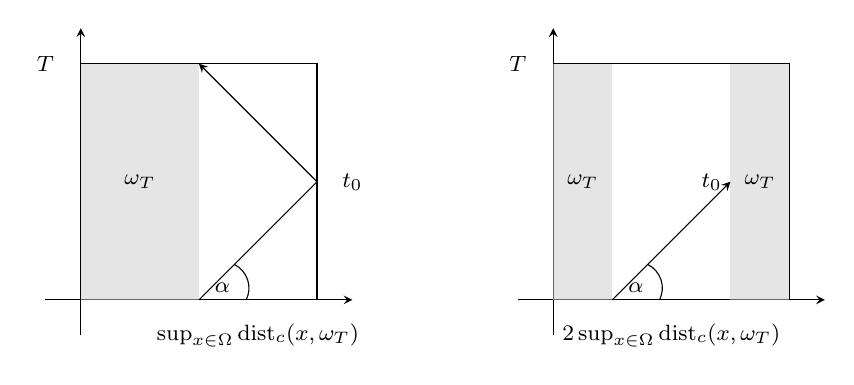
\begin{tikzpicture}[scale=3]
        \draw[-stealth] (-0.15,0) -- (1.15,0); 
        \draw[-stealth] (0,-0.15) -- (0,1.15);
        \draw (0,0) -- (1,0) -- (1,1) -- (0,1) -- cycle;
        \draw[fill=gray!40,draw=none,opacity=0.5] (0,0) -- (0.5,0) -- (0.5,1) -- (0,1) -- cycle;
        \draw[-stealth] (0.5,0) -- (1,0.5) -- (0.5,1);
        \node at (-0.15,1) {\footnotesize $T$}; 
        \node at (0.75,-0.15) {\footnotesize $\sup_{x \in \Omega} \operatorname{dist}_c(x,\omega_T)$}; 
        \node at (1.15,0.5) {\footnotesize $t_0$};
        \draw (0.7,0) to[bend right=45] (0.65,0.15); 
        \node at (0.6,0.05) {\footnotesize $\alpha$};
        \node at (0.25,0.5) {\footnotesize $\omega_T$};
        \begin{scope}[xshift=2cm]
            \draw[-stealth] (-0.15,0) -- (1.15,0); 
            \draw[-stealth] (0,-0.15) -- (0,1.15);
            \draw (0,0) -- (1,0) -- (1,1) -- (0,1) -- cycle;
            \draw[fill=gray!40,draw=none,opacity=0.5] (0,0) -- (0.25,0) -- (0.25,1) -- (0,1) -- cycle;
            \draw[fill=gray!40,draw=none,opacity=0.5] (0.75,0) -- (1,0) -- (1,1) -- (0.75,1) -- cycle;
            \draw[-stealth] (0.25,0) -- (0.75,0.5);
            \node at (-0.15,1) {\footnotesize $T$}; 
            \node at (0.5,-0.15) {\footnotesize $2 \sup_{x \in \Omega} \operatorname{dist}_c(x,\omega_T)$}; 
            \node at (0.67,0.5) {\footnotesize $t_0$};
            \draw (0.45,0) to[bend right=45] (0.4,0.15); 
            \node at (0.35,0.05) {\footnotesize $\alpha$};
            \node at (0.125,0.5) {\footnotesize $\omega_T$};
            \node at (0.875,0.5) {\footnotesize $\omega_T$};
        \end{scope}
    \end{tikzpicture}
    \caption{(\textbf{Can be deleted lateron, only for our own understanding:}) Illustration of the GCC and condition \eqref{eq:Tcondition} in one space dimension. The geometrical setup where the data is given only in one half of the domain is the worst case, because the ray can be reflected at the boundary. We still calculate that $1 = \tan(\alpha) = t_0 / \sup_{x \in \Omega} \operatorname{dist}_c(x,\omega_T)$, i.e. $T > 2 t_0 = 2\sup_{x \in \Omega} \operatorname{dist}_c(x,\omega_T)$ is required for the GCC. Note we can also assume that $c_1 = c_2 = 1$, because the metric is rescaled wrt to the wavespeed. Could probably show that the GCC and the condition on $T$ are in fact equivalent in one dimension.}
\label{fig:GCC-illustration}
\end{figure}


\begin{comment}
\subsubsection{Snell's law... }
\noindent Finally, we consider a more elaborate example. We consider the initial conditions 
\begin{align*}
    u_0 (x,y) &= \frac{1}{100} \exp(-(80(x+y-t-1/5))^2) \vert_{t=0}, \\
    u_1(x,y) &= 128(x+y-t-1/5) \exp(-(80(x+y-t-1/5))^2) \vert_{t = 0}
\end{align*}
and compute a reference solution $u_{\text{ref}}$ numerically. We consider the data domain $\omega_T$ as described in Fig. \ref{fig:2d:SnellsLaw} and presribe $u = \Pi_h u_{\text{ref}}$ on $\omega_T$. 


\newcommand{\hpoint}{0.85}
\begin{figure}
    \centering
    \begin{tikzpicture}[scale=4]
        \draw (0,0) -- (1,0) -- (1,1) -- (0,1) -- cycle;
        \draw[fill=gray!40,draw=none,opacity=0.5] (0,1) -- (0,\hpoint) -- (0.65,\hpoint) -- (0.65,1-\hpoint) -- (0,1-\hpoint) -- (0,0) -- (1,0) -- (1,1) -- cycle;
        \node[draw=none] at (0.85,0.25) {\color{gray} $\omega$};
        \draw[stealth-stealth] (0.7,1-\hpoint) -- (0.7,\hpoint); 
        \node[draw=none] at (0.8,0.5) {\color{black} $h_\omega$};
        \draw[dashed] (0.5,0.5) -- (0,0.5); 
        \draw[-stealth,red,very thick] (0,0.2) -- (0.49,0.5) -- (0,0.8);
        \draw[black,very thick] (0.5,0) -- (0.5,1); 
        \node[draw=none] at (0.55,0.5) {\color{black} $\Gamma$};
        \draw (0.25,0.5) to [bend right=45] (0.25,0.35);
        \node[draw=none] at (0.28,0.44) {\color{black} $\theta_c$};
        \node[draw=none] at (0.5,1.1) {GCC not fulfilled};
        \begin{scope}[xshift=1.25cm]
            \draw (0,0) -- (1,0) -- (1,1) -- (0,1) -- cycle;
            \draw[fill=gray!40,draw=none,opacity=0.5] (0,1) -- (0,0.85*\hpoint) -- (0.65,0.85*\hpoint) -- (0.65,1-0.85*\hpoint) -- (0,1-0.85*\hpoint) -- (0,0) -- (1,0) -- (1,1) -- cycle;
            \draw[stealth-stealth] (0.7,1-0.85*\hpoint) -- (0.7,0.85*\hpoint); 
            \node[draw=none] at (0.8,0.5) {\color{black} $h_\omega$};
            \node[draw=none] at (0.85,0.25) {\color{gray} $\omega$};
            \draw[dashed] (0.5,0.5) -- (0,0.5); 
            \draw[-stealth,red,very thick] (0,0.2) -- (0.49,0.5) -- (0,0.8);
            \draw[black,very thick] (0.5,0) -- (0.5,1); 
            \node[draw=none] at (0.55,0.5) {\color{black} $\Gamma$};
            \draw (0.25,0.5) to [bend right=45] (0.25,0.35);
            \node[draw=none] at (0.28,0.44) {\color{black} $\theta_c$};
            \node[draw=none] at (0.5,1.1) {GCC fulfilled};
        \end{scope}
    \end{tikzpicture}
    \caption{According to Snell's law, rays hitting the interface with an angle greater than the critical angle $\theta_c := \arcsin(\frac{c_1}{c_2})$ are reflected back into the domain $\Omega_1$. To ensure that the GCC is fulfilled, the height $h_{\omega}$ has to chosen smaller than $\tan(\theta_c)$.}
    \label{fig:2d:SnellsLaw}
\end{figure}
\end{comment}


\begin{comment}
\section*{Outtakes}
{\color{gray}
\begin{lem}[Continuity of $A$]
    \begin{enumerate}
        \item For $\Uh \in \ProdFullyDiscrSpace{k}{q}$ and $\mathbf{Y} \in ...$ we have that 
        \begin{equation}
            A[(\Uh,\mathbf{Y})] \le C ... 
        \end{equation}
        \item For $\mathbf{U} \vert_{Q^n} \in ...$ for all $n = 0, \dots, N-1$ and $\Yh \in \ProdFullyDiscrSpace{k^\ast}{q^\ast}$ we have that
        \begin{equation}
            A[(\mathbf{U},\Yh)] \le C ...
        \end{equation}
    \end{enumerate}
\end{lem}

We recall the following interpolation result from \cite{BP24}: 

\begin{lem}[Lem. 2.4 of \cite{BP24}]\label{lem:interpolationOperator}
    Assume that $\Delta t = Ch$ and set $(s,m) = (\min\{k,q\}, \max\{k,q\}+3)$.
    Then, there exists an interpolation operator $\Pi_h$ into $\FullyDiscrSpace{k}{q}$ such that for $n = 0, \dots, N-1$ the following estimates hold
    \begin{enumerate}
        \item $\sum_{n = 0}^{N-1} \{ h^{-1} \Vert u - \Pi_h u \Vert_{L^2(Q^n)} + \Vert \nabla(u - \Pi_h u) \Vert_{L^2(Q^n)} \} \le C \Vert u \Vert_{H^1(Q)}$. 
        \item $\sum_{n = 0}^{N-1} \{ h^{-1} \Vert u - \Pi_h u \Vert_{L^2(Q^n)} + \Vert u - \Pi_h u \Vert_{H^1(Q^n)} \} \le C h^{s} \Vert u \Vert_{H^{m-1}(Q)}$.
        \item $\left( \sum_{n = 0}^{N-1} \int_{I_n} \sum_{K \in \mathcal{T}_h} h^2 \Vert u - \Pi_h u \Vert^2_{H^2(K)} \ \dT \right)^{1/2} \le C h^{s} \Vert u \Vert_{H^{m}(Q)}$ for $u \in H^m(Q_n) \cap C^0(I_n,H^2(\Omega))$.
    \end{enumerate}
\end{lem}



\begin{lem}[Similar to Lem. 2.5 \& Lem. 4.2 of \cite{BP24}]
    In addition to the assumptions of Lem. \ref{lem:interpolationOperator}, let $u \in H^m(Q)$ solve \eqref{eq:waveEquation} and set $\mathbf{U} = (u,\partial_t u)$. Then, the following estimates hold true. 
    \begin{enumerate}
        \item For $u \in H^m(Q) \cap C^0([0,2],H^2(\Omega))$ we have that 
        \begin{equation}
            \vert \mathbf{\Pi}_h \mathbf{U} \vert_{S_h} = \vert \mathbf{\Pi}_h \mathbf{U} - \mathbf{U} \vert_{S_h} \le C h^{s} \Vert u \Vert_{H^m(Q)}.
        \end{equation}
        \item For $u \in H^m(Q)$ we have that
        \begin{equation}
            \vert \mathbf{\Pi}_h \mathbf{U} \vert_{\uparrow \downarrow} \le C h^{s} \Vert u \Vert_{H^{m-1}(Q)}.
        \end{equation}
        \item For $\Uh \in \ProdFullyDiscrSpace{k}{q}$ it holds that 
        \begin{equation}
            \Vert u - \ul_1 \Vert_{\Sigma} + \Vert u - \ul_1 \Vert_{\omega_T} \le C \left( h^{s+1/2} \Vert u \Vert_{H^m(Q)} + \tnorm{(\Uh - \mathbf{\Pi}_h \Uh,0)} \right).
        \end{equation}
        \item For $\mathbf{Y} = (y_1,y_2) \in [H^1(Q)]^2$, we have that
        \begin{equation}
            \Vert \mathbf{\Pi}^\ast_h \mathbf{Y} \Vert_{S_h^\ast} \le C \left( \Vert y_1 \Vert_{H^1(Q)} + \Vert y_2 \Vert_{H^2(Q)} \right). 
        \end{equation}
    \end{enumerate}
\end{lem}

\begin{proof}
    has to be adapted to the current setting.
\end{proof}}

{\color{red} do we need this one? 
\begin{lem}\label{eq:lemma:stability}
    Let $u$ be a solution of \eqref{eq:waveEquation} and $\mathbf{U} = (u,\partial_t u)$. For any $(\Wh,\Yh) \in \ProdFullyDiscrSpace{k}{q} \times \ProdFullyDiscrSpace{k^\ast}{q^\ast}$ it holds that
    \begin{equation*}
        (u - \Pi_h u, \wl_1)_{\omega_T} -  S_h(\mathbf{\Pi}_h \mathbf{U},\Wh) - A[\mathbf{\Pi}_h \mathbf{U},\Yh] - \Sud(\mathbf{\Pi}_h \mathbf{U}, \Wh) \le C h^s \Vert u \Vert_{H^m(Q)} \tnorm{(\Wh,\Yh)}.
    \end{equation*}
\end{lem}

\begin{proof}
    We follow the proof of \cite[Lem. 2.6]{BP24}. 
\end{proof}}
\end{comment}

%\bibliographystyle{alpha}
\bibliography{references}



\end{document}
